\section*{Practice Problems - Fractions}

Convert 22$\dfrac{1}{4}$ into a fraction
Express 10ft, 6in into fraction
Express 10ft, 6in into decimal


\vspace{1cm}
\section*{Practice Problems - Decimals and Powers of Ten}

Write the equivalent of 10,000,000 as a power of ten
Find the product of $3.4564*10^2$
Find the product of $534.567*10^{-2}$
\vspace{0.2cm}
Find the value of $\dfrac{165.93}{10^{-2}}$
\vspace{0.2cm}
Find the value of $0.023*10^4$

\vspace{1cm}
Solutions:\\

$10^7$
345.64
5.34567
16,593
230

\section*{Practice Problems - Rounding and Significant Digits}
Round the following to the nearest hundredths (the second place after the decimal).\\
A. $2.4568$\\
B. $27.2534$\\
C. $128.2111$\\
D. $364.8762$\\
E. $354.777777$\\
F. $34.666666$\\
G. $67.33333$\\
\vspace{0.5cm}
Solution:\\
A. 2.46\\
B. 27.25\\
C. 128.21\\
D. 364.88\\
E. 354.78\\
F. 34.67\\
G. 67.33\\
Round the following to the nearest tenths (the first place after the decimal).\\
A. $2.4568$\\
B. $27.2534$\\
C. $128.2111$\\
D. $364.8762$\\
E. $354.777777$\\
F. $34.666666$\\
G. $67.33333$
Solution:\\
A. 2.5\\
B. 27.3\\
C. 128.2\\
D. 364.9\\
E. 354.8\\
F. 34.7\\
G. 67.3

\vspace{0.5cm}

Round the following answers off to the most significant digit.\\

\begin{tabular}{|l|l|l|}
\hline
 & Problem & Accurate Answer \\
\hline
A. & $25.1+26.43=51.53$ &  \\
\hline
B. & $128.456-121.4=7.056$ &  \\
\hline
C. & $85-7.92432=77.07568$ &  \\
\hline
D. & $8.564+5=13.564$ &  \\
\hline
\end{tabular}

\begin{tabular}{|l|l|l|}
\hline
 & Problem & Accurate Answer \\
\hline
A. & $26.34 \times 124.34567=3,275.26495$ &  \\
\hline
B. & $23.58 \times 34.251=807.63858$ &  \\
\hline
C. & $12,453 / 13.9=895.8992805755$ &  \\
\hline
D. & $12,457.92 \times 3=37,373.76$ &  \\
\hline
\end{tabular}

\section*{Practice Problems - Averages}


Find the average of the following set of numbers:\\
$
\begin{aligned}
&0.2 \\
&0.2 \\
&0.1 \\
&0.3 \\
&0.2 \\
&0.4 \\
&0.6 \\
&0.1 \\
&0.3
\end{aligned}
$

The chemical used for each day during a week is given below. Based on these data, what was the average lb/day chemical used during the week?\\

\begin{tabular}{|l|l|}
\hline
Monday & 92 lb/day\\
\hline
Tuesday & 93 lb/day \\
\hline
Wednesday & 98 lb/day\\
\hline
Thursday & 93 lb/day \\
\hline
Friday & 89 lb/day\\
\hline
Saturday & 93 lb/day \\
\hline
Sunday & 97 lb/day\\
\hline
\end{tabular}

The average chemical use at a plant is 77 lb/day. If the chemical inventory is 2800 lbs, how many days supply is this?

A well pumped for 45 days. The beginning meter reading was 7,456,400 and 45 days later the same meter was 15,154,400. What was the average flow in gallons per day?

\vspace{1cm}

\section*{Practice Problems - Percentage}

$25 \%$ of the chlorine in a 30 -gallon vat has been used. How many gallons are remaining in the vat?

The annual public works budget is $\$ 147,450$. If $75 \%$ of the budget should be spent by the end of September, how many dollars are to be spent? How many dollars will be remaining?

A 75 pound container of calcium hypochlorite has a purity of $67 \%$. What is the total weight of the calcium hypochlorite? 

$3 / 4$ is the same as what percentage?

A $2 \%$ chlorine solution is what concentration in $\mathrm{mg} / \mathrm{L}$ ?

A water plant produces 84,000 gallons per day. 7,560 gallons are used to backwash the filter. What percentage of water is used to backwash?

The average day winter demand of a community is 14,500 gallons. If the summer demand is estimated to be $72 \%$ greater than the winter, what is the estimated summer demand? Demand - When related to use, the amount of water used in a period of time. The term is in reference to the "demand" put onto the system to meet the need of customers.

The master meter for a system shows a monthly total of 700,000 gallons. Of the total water, 600,000 gallons were used for billing. Another 30,000 gallons were used for flushing. On top of that, 15,000 gallons were used in a fire episode and an estimated 20,000 gallons were lost to a main break that was repaired that same day. What is the total unaccounted for water loss percentage for the month?

Your water system takes 75 coliform tests per month. This month there were 6 positive samples. What is the percentage of samples which tested positive?


\vspace{0.3cm}

$Time=\dfrac{Total \enspace volume \enspace to \enspace be \enspace pumped}{Pump \enspace flow \enspace rate}$

\vspace{0.3cm}
$\implies \dfrac{(0.785*110^2*25)\cancel{ft^3}*\dfrac{7.48\cancel{gal}}{\cancel{ft^3}}}{\dfrac{1420\cancel{gal}}{min}}= \boxed{1,251 \enspace min}$\\
\vspace{1cm}
\section*{Practice Problems - Ratio and Proportion}

It takes 6 gallons of chlorine solution to obtain a proper residual when the flow is 45,000 gpd. How many gallons will it take when the flow is 62,000 gpd?

A motor is rated at 41 amps average draw per leg at $30 \mathrm{Hp}$. What is the actual $\mathrm{Hp}$ when the draw is 36 amps? C. 

If it takes 2 operators $4.5$ days to clean an aeration basin, how long will it take three operators to do the same job?

It takes 3 hours to clean 400 feet of collection system using a sewer ball. How long will it take to clean 250 feet?

It takes 14 cups of $\mathrm{HTH}$ to make a $12 \%$ solution, and each cup holds 300 grams. How many cups will it take to make a $5 \%$ solution?

A bike travelling at 5 miles/hr completes a journey in 40 minutes. How long would the same journey take if the speed was increased to 8 miles/hr?

\vspace{1cm}

\textbf{Solution}

The gallons chlorine and flow are directly related. 

Thus,

$\dfrac{6}{45,000}=\dfrac{X}{62,000} \implies X=\dfrac{6*62,000}{45,000}=8.3 \mathrm{gallons}$


\vspace{0.5cm}

The amp draw and Hp are directly related.

This

$\dfrac{30}{41}=\dfrac{X}{36} \implies X=\dfrac{30*36}{41}=26.3 \mathrm{Hp}$

\vspace{0.5cm}

The number of operators and the days to clean are inversely related.

Thus,

$2 * 4.5 = 3*X \implies X = \dfrac{2*4.5}{3} = 3 \mathrm{days}$



\vspace{0.5cm}

The hours to clean and the length of system cleaned are directly proportional.

Thus,

$\dfrac{3}{400}=\dfrac{X}{250} \implies X=\dfrac{3*250}{400}=1.9 \mathrm{hours}$

\vspace{0.5cm}

The cups of HTH and percentage HTH solution are directly proportional.

Thus,

$\dfrac{14}{12}=\dfrac{X}{5} \implies X=\dfrac{14*5}{12}=5.8 \mathrm{cups}$

\vspace{0.3cm}

The bike speed and time to complete the journey are inversely related.

Thus,

$5 * 40 = 8*X \implies X = \dfrac{5*40}{8} = 25 \mathrm{min}$



\vspace{1cm}
\section*{Practice Problems - Area and Volume}


A 60-foot diameter tank contains 422,000 gallons of water. Calculate the height of water in the storage tank.

What is the volume of water in ft$^3$, of a sedimentation basin that is 22 feet long, and 15 feet wide, and filled to 10 feet?

What is the volume in ft$^3$ of an elevated clear well that is 17.5 feet in diameter, and filled to 14 feet?

What is the area of the top of a storage tank that is 75 feet in diameter?\\

 What is the area of a wall $175 \mathrm{ft}$. in length and $20 \mathrm{ft}$. wide?\\

 You are tasked with filling an area with rock near some of your equipment. 1 Bag of rock covers 250 square feet. The area that needs rock cover is 400 feet in length and 30 feet wide. How many bags do you need to purchase?\\

A circular clearwell is 150 feet in diameter and 40 feet tall. The Clearwell has an overflow at 35 feet. What is the maximum amount of water the clearwell can hold in Million gallons rounded to the nearest hundredth?\\


 A sedimentation basin is 400 feet length, 50 feet in width, and 15 feet deep. What is the volume expressed in cubic feet?\\


 A clearwell holds $314,000 \mathrm{ft}^{3}$ of water. It is $100 \mathrm{ft}$ in diameter. What is the height of the clearwell?\\

 A treatment plant operator must fill a clearwell with $10,000 \mathrm{ft}^{3}$ of water in 90 minutes. What is the rate of flow expressed in GPM?\\


 A water tank has a capacity of 6MG. It is currently half full. It will take 6 hours to fill. What is the flow rate of the pump?\\


 A clearwell with the capacity of $2.5 \mathrm{MG}$ is being filled after a maintenance period. The flow rate is 2,500 GPM. The operator begins filling at 7 AM. At what time will the clearwell be full?\\

  A chemical feed pump with a 6-inch bore and a 6-inch stroke pumps 60 cycles per minute. Find the pumping rate in gpm.
  
  Determine the flow capacity of a pump in gpm if the pump lowers the water level in a 6 -foot square wet well by 8 inches in 5 minutes.
  
  A new 6" diameter pipeline is installed with a length of 7,000 feet and a depth-to-invert of 6 feet. The trench must be excavated with walls 2 feet wider than the pipe on each and 6" below the invert.  The trench will be backfilled with slurry. All the native material must be hauled away. How many cubic yards of native material are removed from the trench.  (Ans: 11,792 cu. yds)
  
A 12" diameter pipe is to be installed 4 feet deep (to top-of-pipe) with a length of 15,000 feet. The area around the pipe will be backfilled with sand. The area around the pipe includes bedding and shading requirements that are each 6". The trench walls are one foot wider than the pipe on each side. How much sand is required in cubic yards? (Ans: 2,897 cu. yds)

A new 24" diameter pipe is to be installed with a pipe depth, to top of pipe, of 48" and a length of 12,000 feet
The trench will be backfilled with sand. The trench walls will be excavated one foot wider than the pipe on each side and six inches below the pipe.  A) How much excavated material must be hauled away?  (Ans: 11,555 cu. yds) B) How much sand is required to backfill the trench to an asphalt subgrade that is 12" below the street surface. (Ans: 6,949 cu. yds)

How much paint will it take for a single coat of the top and sidewalls of the storage tank that is 100-feet in diameter and 30-feet tall, if one gallon of paint covers 200 square feet?\\
a. $\quad 86$ gallons\\
b. $\quad 96$ gallons\\
c. $\quad 106$ gallons\\
d. $\quad 116$ gallons\\
e. $\quad 126$ gallons

Under like conditions, how much more water would an 8-inch pipe carry than a 4-inch pipe?\\
a.	2 times\\
b.	3 times\\
c.	4 times\\
d.	not enough information given\\





\textbf{Solution:}\\


Volume = Surface area * height $\implies \mathrm{height}=\dfrac{\mathrm{Volume}}{\mathrm{Surface \enspace area}}$\\
\vspace{0.2cm}

\begin{tikzpicture}
\draw (0,0) ellipse (2cm and 0.3cm);
\draw (0,-2.3) ellipse (2cm and 0.3cm);
\draw [-] (2,-2.3) -- (2,0);
\draw [<->] (-2,0) -- (2,0) node [midway, above=3mm] {\hspace{0.1cm}Diameter=60'}; 
\draw [<->] (2.5,-2.3) -- (2.5,0) node [midway, below] {\hspace{1.9cm}Height=h'};
%\draw [-] (0,-4) -- (2,-2.3);
%\draw [-] (0,-4) -- (-2,-2.3);
%\draw [-] (0,-4) -- (2,-2.3);
\draw [-] (-2,0) -- (-2,-2.3);
\draw (0,-1.2) node[text width=4cm,align=center]
  {Volume=422,000 gal};
\end{tikzpicture}\\
\vspace{0.2cm}
$\implies \mathrm{height}=\dfrac{422,000 \enspace \cancel{\mathrm{gal}}*\dfrac{\cancelto{\mathrm{ft}}{\mathrm{ft}^3}}{7.48 \enspace \cancel{\mathrm{gal}}}}{0.785*60^2 \enspace \cancel{\mathrm{ft^2}}}=\boxed{101 \enspace \mathrm{ft}}$



\vspace{1cm}
\section*{Practice Problems - Flow and Velocity}


A rectangular channel 3 ft. wide contains water 2 ft. deep flowing at a velocity of 1.5 fps.
What is the flow rate in cfs?

Flow in an 8-inch pipe is 500 gpm. What is the average velocity in ft/sec? (Assume pipe is flowing full)

A pipeline is 18” in diameter and flowing at a velocity of 125 ft. per minute. What is the flow in gallons per minute?

The velocity in a pipeline is 2 ft./sec. and the flow is 3,000 gpm. What is the diameter of the pipe in inches?



Find the flow in a 4-inch pipe when the velocity is $1.5$ feet per second.

  A 42-inch diameter pipe transfers 35 cubic feet of water per second. Find the velocity in $\mathrm{ft} / \mathrm{sec}$. 
  
  A plastic float is dropped into a channel and is found to travel 10 feet in $4.2$ seconds. The channel is $2.4$ feet wide and $1.8$ feet deep. Calculate the flow rate of water in cfs.

  The flow velocity of a 6-inch diameter pipe is twice that of a 12-inch diameter pipe if both are carrying 50 gpm of water. True or false?

  What should the flow meter read in gpm if a 4-inch diameter main is to be flushed at a velocity of $4.6$ fps?

  The velocity through a channel is $4.18$ fps. If the channel is 4 feet wide by 2 feet deep by 10 feet long, what is the flow rate in gpm?

  What is the average flow velocity in $\mathrm{ft} / \mathrm{sec}$ for a 12-inch diameter main carrying a daily flow of $2.5 \mathrm{mgd}$ ?





\textbf{Solution:}\\



Solution:\\
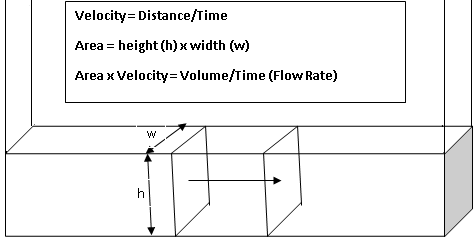
\includegraphics[scale=0.5]{ChannelFlow3}\\
$Q=V*A \implies Q = 1.5 \dfrac{ft}{sec}*(3*2)ft^2=\boxed{9\dfrac{ft^3}{sec}}$

Solution:\\
\vspace{0.5cm}
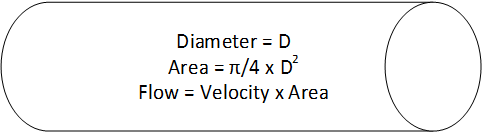
\includegraphics[scale=0.5]{PipeFlow}\\
$Q=V*A$\\
$\implies V=\dfrac{Q}{A} \implies V \Big(\dfrac{ft}{s}\Big)= \dfrac{\dfrac{500\cancel{gallon}}{\cancel{min}}*\dfrac{\cancelto{ft}{ft^3}*\dfrac{min}{60sec}}{7.48\cancel{gal}}}{0.785*\Big(\dfrac{8}{12}\Big)^2\cancelto{}{ft^2}}=\boxed{3.2ft/s}$

Solution:\\

\vspace{0.5cm}

The diameter of the pipe is 4 inches. Therefore, the radius is 2 inches. Convert the 2 inches to feet.
$
\begin{aligned}
&\dfrac{2}{12}=0.6667 \mathrm{ft} \\
&\mathrm{A}=\pi \times \mathrm{r}^{2} \\
&\mathrm{~A}=\pi \times(0.167 \mathrm{ft})^{2} \\
&\mathrm{~A}=\pi \times 0.028 \mathrm{ft}^{2} \\
&\mathrm{~A}=0.09 \mathrm{ft}^{2} \\
&\mathrm{Q}=\mathrm{V} \times \mathrm{A} \\
&\mathrm{Q}=1.5 \mathrm{ft} / \mathrm{sec} \times 0.09 \mathrm{ft}^{2} \\
&\mathrm{Q}=0.14 \mathrm{ft} / 3 \mathrm{sec}(\mathrm{cfs})
\end{aligned}
$



\vspace{1cm}

\vspace{1cm}

\section*{Practice Problems - Unit Conversions}
Convert the following:\\

Convert 1000 $ft^3$ to cu. yards\\

Convert 10 gallons/min to $ft^3$/hr\\

Convert 100,000 $ft^3$ to acre-ft.\\

Find the flow in gpm when the total flow for the day is 65,000 gpd.

Find the flow in gpm when the flow is $1.3 \mathrm{cfs}$.

Find the flow in gpm when the flow is $0.25 \mathrm{cfs}$.

The flow rate through a filter is 4.25 MGD. What is this flow rate expressed as gpm?\\

After calibrating a chemical feed pump, you've determined that the maximum feed rate is $178 \mathrm{~mL} /$ minute. If this pump ran continuously, how many gallons will it pump in a full day?

A plant produces 2,000 cubic foot of water per hour. How many gallons of water is produced in an 8-hour shift?

Change 70 °F to °C
Change 140 °F to °C
Change 20 °C to °F
Change 85 °C to °F
Change 4 °C to °F

\textbf{Solution}

Solution:\\

$1000 \cancel{ft^3}*\dfrac{cu.yards}{27\cancel{ft^3}} = 37 cu.yards$

Solution:\\

\vspace{0.4cm}

$\dfrac{10 \enspace \cancel{\mathrm{gallons}}}{\cancel{\mathrm{min}}}*  \dfrac{\mathrm{ft}^3}{7.48 \cancel{\mathrm{gallons}}}  * \dfrac{60 \cancel{\mathrm{min}}}{\mathrm{hr}}   = \dfrac{80.2 \enspace \mathrm{ft}^3}{\mathrm{hr}}$

\vspace{0.4cm}


Solution:\\

\vspace{0.4cm}

$100,000 \cancel{ft^3} * \dfrac{acre-ft}{43,560 \cancel{ft^2-ft}} =  2.3 acre-ft$\\

\vspace{0.2cm}

\textbf{Note:} From the conversion table: acre = 43,560 $ft^2$\\
Thus, acre-ft  = 43,560 $ft^2$-ft or 43,560 $ft^3$\\

\vspace{0.4cm}

Solution:\\

\vspace{0.4cm}

$
\dfrac{65,000 \mathrm{gpd}}{1,440 \mathrm{~min} / \mathrm{day}}=45 \mathrm{gpm}
$

\vspace{0.4cm}

Solution:\\
$
1.3 \dfrac{\mathrm{cfs}}{1} \mathrm{x} \dfrac{448 \mathrm{gpm}}{1 \mathrm{cfs}}=582 \mathrm{gpm}
$

\vspace{0.4cm}

Solution:\\

\vspace{0.4cm}

$
0.25 \dfrac{\mathrm{cfs}}{1} \times \dfrac{448 \mathrm{gpm}}{1 \mathrm{cfs}}=112 \mathrm{gpm}
$

\vspace{0.4cm}

Solution:\\

\vspace{0.2cm}

$Flow rate, gpm=\dfrac{Flow \enspace rate, \enspace gpd}{1440 \enspace min/day}$\\

\vspace{0.2cm}

Note:  We are assuming that the filter operated uniformly over that 24 hour period.\\

\vspace{0.3cm}

$Flow rate, gpm=\dfrac{4.25 \enspace \dfrac{\cancel{MG}}{\cancel{day}} *1,000,000 \enspace \dfrac{gal}{\cancel{MG}}}{1440\dfrac{min}{\cancel{day}}}=\boxed{2,951 \enspace gpm}$


Solution:\\

\vspace{0.4cm}

$\dfrac{2000 \enspace \cancel{\mathrm{ft}^3}}{\cancel{hr}}*  \dfrac{7.48 \enspace{\mathrm{gallons}}}{\cancel{\mathrm{ft}^3}}  * \dfrac{60 \enspace \cancel{\mathrm{hr}}}{\mathrm{shift}}   = \boxed{\dfrac{119,680 \enspace \mathrm{gallons}}{\mathrm{shift}}}$

\vspace{0.4cm}



\vspace{1cm}

\section*{Practice Problems - Concentration}

What is the concentration in mg/l of  4.5\% solution of that substance.

How many lbs of salt is needed to make 5 gallons of a 2,500mg/l solution


\vspace{0.5cm}
\textbf{Solution}\\

45,000 mg/l

Applying pounds formula:  lbs salt = $\dfrac{5}{1,000,000}*2,500*8.34=\boxed{0.14lbs}$



\vspace{1cm}
\section*{Practice Problems - Density and Specific Gravity}


What is the specific gravity of a 1 ft$^3$ concrete block which weighs 145 lbs?

What is the specific gravity of a chlorine solution if 1 (one) gallon weighs 10.2lbs?

How much does each gallon of zinc orthophosphate weigh (pounds) if it has a specific gravity of 1.46?

How much does a 55 gallon drum of 25\% caustic soda weigh (pounds) if the specific gravity is 1.28?



\section*{Practice Problems - Detention Time}

A flocculation basin is 7 ft deep, 15 ft wide, and 30 ft long. If the flow through the basin is 1.35 MGD, what is the detention time in minutes?

A tank has a diameter of 60 feet with an overflow depth at 44 feet. The current water level is 16 feet. Water is flowing into the tank at a rate of 250 gallons per minute. At this rate, how many days will it take to fill the tank to the overflow?

How long will it take to fill a 50 gallon hypochlorite tank if the flow is $5 \mathrm{gpm}$ ?

Find the detention time in a 45,000 gallon reservoir if the flow rate is $85 \mathrm{gpm}$.

If the fuel consumption to the boiler is 35 gallons per day. How many days will the 500 gallon tank last.

The sedimentation basin on a water plant contains 5,775 gallons. What is the detention time if the flow is $175 \mathrm{gpm}$.


\textbf{Solution}\\

Solution:\\
\vspace{0.5cm}
\begin{tikzpicture}

\pgfmathsetmacro{\cubexx}{4}
\pgfmathsetmacro{\cubeyy}{1.5}
\pgfmathsetmacro{\cubezz}{2}
\pgfmathsetmacro{\cubex}{4}
\pgfmathsetmacro{\cubey}{0.5}
\pgfmathsetmacro{\cubez}{2}
\filldraw [fill=lightgray!20, draw=black] (0,-\cubey,0) -- ++(-\cubexx,0,0) -- ++(0,-\cubeyy,0) -- ++(\cubexx,0,0) -- cycle ;
\filldraw [fill=lightgray!20, draw=black] (0,-\cubey,0) -- ++(0,0,-\cubezz) -- ++(0,-\cubeyy,0) -- ++(0,0,\cubezz) -- cycle;
\filldraw [fill=lightgray!20, draw=black] (0,-\cubey,0) -- ++(0,0,-\cubezz) -- ++(0,-\cubeyy,0) -- ++(0,0,\cubezz) -- cycle;
\filldraw [fill=lightgray!20, draw=black] (0,-\cubey,0) -- ++(-\cubexx,0,0) -- ++(0,0,-\cubezz) -- ++(\cubexx,0,0) -- cycle;
%\draw (0,-0.5,0) -- ++(-\cubex,0,0) -- ++(0,-\cubey,-\cubez) -- ++(\cubex,0,0) -- cycle;
\draw (-\cubex,0,0) -- ++(0,0,-\cubez) -- ++(0,-\cubey,0) -- ++(0,0,\cubez) -- cycle;
\draw (0,-\cubey,0) -- ++(-\cubex,0,0) -- ++(0,0,-\cubez) -- ++(\cubex,0,0) -- cycle;




\filldraw [fill=white, draw=black] (0,0,0) -- ++(-\cubex,0,0) -- ++(0,-\cubey,0) -- ++(\cubex,0,0) -- cycle ;
\filldraw [fill=white, draw=black] (0,0,0) -- ++(0,0,-\cubez) -- ++(0,-\cubey,0) -- ++(0,0,\cubez) -- cycle;
\filldraw [fill=white, draw=black] (0,0,0) -- ++(0,0,-\cubez) -- ++(0,-\cubey,0) -- ++(0,0,\cubez) -- cycle;
\filldraw [fill=white, draw=black] (0,0,0) -- ++(-\cubex,0,0) -- ++(0,0,-\cubez) -- ++(\cubex,0,0) -- cycle;
%\draw (0,-0.5,0) -- ++(-\cubex,0,0) -- ++(0,0,-\cubez) -- ++(\cubex,0,0) -- cycle;
%\filldraw [fill=white, draw=black] (-\cubex,0,0) -- ++(0,0,-\cubez) -- ++(0,-\cubey,0) -- ++(0,0,\cubez) -- cycle;
%\filldraw [fill=white, draw=black] (0,-\cubey,0) -- ++(-\cubex,0,0) -- ++(0,0,-\cubez) -- ++(\cubex,0,0) -- cycle;

\draw [<->] (-4,-2.3) -- (0,-2.3) node [midway, below] {\scriptsize{30' long}};
\draw [<->] (1,-1.3) -- (1,.2) node [midway, below] {\hspace{2.2cm}\scriptsize{7' deep}};
%\draw [<->] (1,.8) -- (1,.2) node [midway, below] {\hspace{2.2cm}Text Y Axis};
\draw [<->] (1,-1.3) -- (0,-2.3) node [midway, below] {\hspace{1.7cm}\scriptsize{15' wide}};
\draw [->](-6,-1) -- (-4,-1) node [midway, above] {\hspace{0.5cm}\scriptsize{1.5 MGD}};
\draw [->](0.3,-1) -- (0.9,-1) node [midway, above] {};
\end{tikzpicture}\\

\vspace{0.4cm}
$
\mathrm{DT}=\dfrac{(30*15*7) \mathrm{ft^3}*7.48\dfrac{gal}{ft^3}}{1,350,000 \dfrac{\mathrm{gal}}{day}*\dfrac{\mathrm{day}}{1440\mathrm{min}}}=25 \mathrm{min}
$


\vspace{0.4cm}


Solution:\\

\vspace{0.4cm}
\begin{tikzpicture}[scale=1]
\node [draw, cylinder, cylinder uses custom fill, cylinder body fill=green!20, 
cylinder end fill=green!20, shape aspect=4, rotate=90, minimum width=3cm] (c1) at 
(0,1.8){};

\coordinate(dhtop) at ($(c1.after top)!-1*.1!(c1.before top)$);
\coordinate(dhbot) at ($(c1.before bottom)!-1*.1!(c1.after bottom)$);
\coordinate(dhlabel) at ($(dhtop)!.5!(dhbot)$);
%\draw[|-|] (dhbot)--(dhtop);
%\path (dhlabel) node[right, outer sep = 2pt] {$44'$};

\node [draw, cylinder, cylinder body fill=black!20, cylinder end fill=red!20, shape aspect=4, rotate=90, minimum height=4cm, minimum width=3cm] (c) {};

\coordinate(htop) at ($(c.before top)!-1*.1!(c.after top)$);
\coordinate(hbot) at ($(c.after bottom)!-1*.1!(c.before bottom)$);
\coordinate(hlabel) at ($(htop)!.5!(hbot)+(c.north)!.9!(c.center)$);

%\draw[|-|] (hbot)--(htop);
%\path (hlabel) node[left] {}; %Modify height label here


%\node [draw, cylinder, cylinder uses custom fill, cylinder body fill=black!20, 
%cylinder end fill=lightgray!20, shape aspect=4, rotate=90, minimum width=3cm] (c1) at 
%(0,3.8){};


\node [draw, cylinder, cylinder uses custom fill, cylinder body fill=black!20, 
cylinder end fill=lightgray!20, shape aspect=4, rotate=90, minimum width=3cm] (c1) at 
(0,-1.2){};

%\node [draw, cylinder, cylinder uses custom fill, cylinder body fill=blue!20, 
cylinder end fill=green!20, shape aspect=4, rotate=90, minimum width=3cm] (c1) at 
(0,0){};

%\coordinate (center) at ($(c.before top)!0.5!(c.after top)$);
%\filldraw (center) circle (1pt);
%
%\coordinate (rlabel) at ($(center) !0.5!(c.after top)$);
%\coordinate (rtop) at ($(center)!-1*.1!(c.after top)$);

%\coordinate (rend) at ($(c.mid east)!0.5!(c.after top)$);
%\draw[-, shorten >=-10] (center) -- (rend);
%\path (rend) node[outer sep = 5pt, left] {$r$};
\draw [<->] (-1.5,2.4) -- (1.5,2.4) node [midway, above=1mm] {\hspace{0.05cm}\scriptsize{Diameter=60'}};
%\draw [<->] (1.8,2.4) -- (1.8,1.9) node [midway, midway] {\hspace{2.4cm}\scriptsize{16' Freeboard}};
%\draw [<->] (1.8,1.9) -- (1.8,-0.7) node [midway, midway] {\hspace{2.4cm}\scriptsize{28' Fill}};
%\draw [<->] (1.8,-1.1) -- (1.8,-0.7) node [midway, midway] {\hspace{2.8cm}\scriptsize{16' Current Level}};
\draw (3.3,1.9) node{\scriptsize{Overflow level = 44'}};
\draw (3.22,-0.6) node{\scriptsize{Current level = 16'}};
\draw [<-] (1.5,-0.6) -- (2.2,-0.6);
\draw [<-] (1.5,1.9) -- (2.2,1.9);
\draw[thick,->](0,3.5)--(0,2.5) node [at start, above, black] (n){\scriptsize{250 gpm}};
\end{tikzpicture}

$\mathrm{Fill \enspace time}=\dfrac{Volume}{Flow}=\dfrac{0.785*60^2*(44-16)ft^3*\dfrac{7.48 gallons}{ft^3}}{250 \dfrac{gallons}{min}*\dfrac{1440 \enspace min}{day}}=1.6 \enspace days$
\vspace{0.4cm}

Solution:\\4

\vspace{0.4cm}



\vspace{0.4cm}

Solution:\\5

\vspace{0.4cm}

$
\mathrm{DT}=\dfrac{50 \mathrm{gal}}{5 \mathrm{gal} / \mathrm{min}}=10 \mathrm{~min}
$

\vspace{0.4cm}

Solution:\\

\vspace{0.4cm}

$
\mathrm{DT}=\dfrac{45,000 \mathrm{gal}}{85 \mathrm{gal} / \mathrm{min}}=529 \mathrm{~min} \quad \text { or } \dfrac{529 \mathrm{~min}}{60 \mathrm{~min} / \mathrm{hr}}=8.8 \mathrm{hrs}
$
\vspace{0.4cm}

Solution:\\

\vspace{0.4cm}

$
\mathrm{DT}=\dfrac{500 \text { gal }}{35 \mathrm{gal} / \text { day }}=14.3 \text { days }
$
\vspace{0.4cm}

Solution:\\

\vspace{0.4cm}

$
\mathrm{DT}=\dfrac{5,775 \mathrm{gal}}{175 \mathrm{gal} / \mathrm{min}}=33 \mathrm{~min}
$


\vspace{1cm}

\section*{Practice Problems - Unit Conversions}

Convert 22\degree{C} into degree Fahrenheit.
Convert 56\degree{C} into degree Celsius.

\vspace{1cm}

\section*{Practice Problems - Pounds Formula}


A water treatment plant operates at the rate of 75 gallons per minute. They dose soda ash at
14 mg/L. How many pounds of soda ash will they use in a day?

A water treatment plant is producing 1.5 million gallons per day of potable water, and
uses 38 pounds of soda ash for pH adjustment. What is the dose of soda ash at that plant?

A water treatment plant produces 150,000 gallons of water every day. It uses an
average of 2 pounds of permanganate for iron and manganese removal. What is the dose of the
permanganate? 

A water treatment plant uses 8 pounds of chlorine daily and the dose is 17 mg/l. How
many gallons are they producing?

An operator mixes 40 lb of lime in a 100-gal tank containing 80 gal of water. What is the percent of lime in the slurry?

A treatment plant has a maximum output of $30 \mathrm{MGD}$ and doses ferric chloride at 75 $\mathrm{mg} / \mathrm{L}$. How many pounds of Ferric Chloride does the plant use in a day?\\

 A treatment plant uses 750 pounds of alum a day as it treats $15 \mathrm{MGD}$. What was the dose rate?\\


 A treatment plant operates at 1,500 gallons a minute and uses 500 pounds of alum a day. What is the alum dose?\\



\textbf{Solution:}
[1.]
Solution:\\

\begin{figure}[h]
\begin{tikzpicture}
    \newcommand{\R}{1.5}

\path[help lines,step=.2] (0,0) grid (16,3);
\path[help lines,line width=.6pt,step=1] (0,0) grid (16,3);
%\foreach \x in {0,1,2,3,4,5,6,7,8,9,10,11,12,13,14,15,16}
%\node[anchor=north] at (\x,0) {\x};
%\foreach \y in {0,1,2,3,4,5,6}
%\node[anchor=east] at (0,\y) {\y};
%-------------CIRCLE-----------------------------------
\draw[black,fill=gray!10] (8,3) circle (\R);
\draw[black, very thick, rotate=0](6.5,3) -- (9.5,3);
\draw (8,3.6) node[text width=3cm,align=center]
  {\scriptsize{lbs/day}};
\draw (7.1,2.5) node[text width=3cm,align=center]
  {\tiny{14 mg/l}};
\draw (8.9,2.5) node[text width=3cm,align=center]
  {\tiny{75 GPM}};
  \draw (8,2)node[text width=3cm,align=center]
  {\tiny{8.34}};
\draw[black, very thick, rotate=0](7.2,1.7) -- (8,3);
\draw[black, very thick, rotate=0](8.8,1.7) -- (8,3);
\end{tikzpicture}
\end{figure}
$\dfrac{\mathrm{lbs}}{\mathrm{day}}=\mathrm{Flow}\dfrac{{\mathrm{MG}}}{\mathrm{day}}* \mathrm{Concentration}\dfrac{\mathrm{mg}}{\mathrm{l}}*8.34$
\\
\vspace{0.2cm}
$\dfrac{\mathrm{lbs}}{\mathrm{day}}=75 \dfrac{\cancel{\mathrm{gallons}}}{\cancel{\mathrm{min}}}* 1440\dfrac{\cancel{\mathrm{min}}}{\mathrm{day}}*\dfrac{\mathrm{MG}}{1,000,000 \enspace \cancel{\mathrm{gallons}}}*250\dfrac{\mathrm{mg}}{\mathrm{l}}*8.34 = \boxed{225\dfrac{lbs}{day}}$
\vspace{0.2cm}
 Solution:\\
 \begin{figure}[h!]
\begin{tikzpicture}
    \newcommand{\R}{1.5}

\path[help lines,step=.2] (0,0) grid (16,3);
\path[help lines,line width=.6pt,step=1] (0,0) grid (16,3);
%\foreach \x in {0,1,2,3,4,5,6,7,8,9,10,11,12,13,14,15,16}
%\node[anchor=north] at (\x,0) {\x};
%\foreach \y in {0,1,2,3,4,5,6}
%\node[anchor=east] at (0,\y) {\y};
%-------------CIRCLE-----------------------------------
\draw[black,fill=gray!10] (8,3) circle (\R);
\draw[black, very thick, rotate=0](6.5,3) -- (9.5,3);
\draw (8,3.6) node[text width=3cm,align=center]
  {\scriptsize{38 lbs/day}};
\draw (7.1,2.5) node[text width=3cm,align=center]
  {\tiny{? mg/l}};
\draw (8.9,2.5) node[text width=3cm,align=center]
  {\tiny{1.5 MGD}};
  \draw (8,2)node[text width=3cm,align=center]
  {\tiny{8.34}};
\draw[black, very thick, rotate=0](7.2,1.7) -- (8,3);
\draw[black, very thick, rotate=0](8.8,1.7) -- (8,3);
\end{tikzpicture}
\end{figure}
$\dfrac{\mathrm{lbs}}{\mathrm{day}}=\mathrm{Flow}\dfrac{{\mathrm{MG}}}{\mathrm{day}}* \mathrm{Concentration}\dfrac{\mathrm{mg}}{\mathrm{l}}*8.34 \hspace{0.2cm} \implies \mathrm{Concentration}\dfrac{\mathrm{mg}}{\mathrm{l}}=\dfrac{ \dfrac{\mathrm{lbs}}{\mathrm{day}}}{\mathrm{Flow}\dfrac{{\mathrm{MG}}}{\mathrm{day}}*8.34}$
\vspace{0.2cm}
$\mathrm{Concentration}\dfrac{\mathrm{mg}}{\mathrm{l}}=\dfrac{ 38\dfrac{\mathrm{lbs}}{\mathrm{day}}}{1.5\dfrac{{\mathrm{MG}}}{\mathrm{day}}*8.34}=\boxed{3\dfrac{\mathrm{mg}}{\mathrm{l}}}$
\\
\vspace{0.2cm}



 Solution:\\
 \begin{figure}[h!]
\begin{tikzpicture}
    \newcommand{\R}{1.5}

\path[help lines,step=.2] (0,0) grid (16,3);
\path[help lines,line width=.6pt,step=1] (0,0) grid (16,3);
%\foreach \x in {0,1,2,3,4,5,6,7,8,9,10,11,12,13,14,15,16}
%\node[anchor=north] at (\x,0) {\x};
%\foreach \y in {0,1,2,3,4,5,6}
%\node[anchor=east] at (0,\y) {\y};
%-------------CIRCLE-----------------------------------
\draw[black,fill=gray!10] (8,3) circle (\R);
\draw[black, very thick, rotate=0](6.5,3) -- (9.5,3);
\draw (8,3.6) node[text width=3cm,align=center]
  {\scriptsize{38 lbs/day}};
\draw (7.1,2.5) node[text width=3cm,align=center]
  {\tiny{? mg/l}};
\draw (8.9,2.5) node[text width=3cm,align=center]
  {\tiny{1.5 MGD}};
  \draw (8,2)node[text width=3cm,align=center]
  {\tiny{8.34}};
\draw[black, very thick, rotate=0](7.2,1.7) -- (8,3);
\draw[black, very thick, rotate=0](8.8,1.7) -- (8,3);
\end{tikzpicture}
\end{figure}
$\dfrac{\mathrm{lbs}}{\mathrm{day}}=\mathrm{Flow}\dfrac{{\mathrm{MG}}}{\mathrm{day}}* \mathrm{Concentration}\dfrac{\mathrm{mg}}{\mathrm{l}}*8.34 \hspace{0.2cm} \implies \mathrm{Concentration}\dfrac{\mathrm{mg}}{\mathrm{l}}=\dfrac{ \dfrac{\mathrm{lbs}}{\mathrm{day}}}{\mathrm{Flow}\dfrac{{\mathrm{MG}}}{\mathrm{day}}*8.34}$
\vspace{0.2cm}
$\mathrm{Concentration}\dfrac{\mathrm{mg}}{\mathrm{l}}=
\dfrac{ 2\dfrac{\mathrm{lbs}}{\mathrm{day}}}
{\Bigg(150,000 \dfrac{\cancel{\mathrm{Gallons}}}
{\mathrm{day}}*
\dfrac{\mathrm{MG}}
{1,000,000 \cancel{\enspace \mathrm{Gallons}}}*8.34\Bigg)}
=\boxed{3\dfrac{\mathrm{mg}}{\mathrm{l}}}$
\\
\vspace{0.2cm}


 Solution:\\
 \begin{figure}[h!]
\begin{tikzpicture}
    \newcommand{\R}{1.5}

\path[help lines,step=.2] (0,0) grid (16,3);
\path[help lines,line width=.6pt,step=1] (0,0) grid (16,3);
%\foreach \x in {0,1,2,3,4,5,6,7,8,9,10,11,12,13,14,15,16}
%\node[anchor=north] at (\x,0) {\x};
%\foreach \y in {0,1,2,3,4,5,6}
%\node[anchor=east] at (0,\y) {\y};
%-------------CIRCLE-----------------------------------
\draw[black,fill=gray!10] (8,3) circle (\R);
\draw[black, very thick, rotate=0](6.5,3) -- (9.5,3);
\draw (8,3.6) node[text width=3cm,align=center]
  {\scriptsize{8 lbs/day}};
\draw (7.1,2.5) node[text width=3cm,align=center]
  {\tiny{17 mg/l}};
\draw (8.9,2.5) node[text width=3cm,align=center]
  {\tiny{? MGD}};
  \draw (8,2)node[text width=3cm,align=center]
  {\tiny{8.34}};
\draw[black, very thick, rotate=0](7.2,1.7) -- (8,3);
\draw[black, very thick, rotate=0](8.8,1.7) -- (8,3);
\end{tikzpicture}
\end{figure}
$\dfrac{\mathrm{lbs}}{\mathrm{day}}=\mathrm{Flow}\dfrac{{\mathrm{MG}}}{\mathrm{day}}* \mathrm{Concentration}\dfrac{\mathrm{mg}}{\mathrm{l}}*8.34 \hspace{0.2cm}$\\
\vspace{0.2cm}
$\implies \mathrm{Flow}\dfrac{{\mathrm{MG}}}{day}=\dfrac{ \dfrac{\mathrm{lbs}}{\mathrm{day}}}{\mathrm{Concentration}\dfrac{\mathrm{mg}}{\mathrm{l}}*8.34}=\dfrac{8 \dfrac{\mathrm{lbs}}{\mathrm{day}}}{17\dfrac{\mathrm{mg}}{\mathrm{l}}*8.34}=0.056425\dfrac{{\mathrm{MG}}}{day}$\\
\vspace{0.2cm}
$0.056425\dfrac{{\mathrm{MG}}}{day}*\dfrac{1,000,000 \enspace \mathrm{Gallons}}{\mathrm{MG}}=\boxed{56,425 \enspace \mathrm{Gallons}}$
\vspace{0.2cm}


 Solution:\\
 \begin{figure}[h!]
\begin{tikzpicture}
    \newcommand{\R}{1.5}

\path[help lines,step=.2] (0,0) grid (16,3);
\path[help lines,line width=.6pt,step=1] (0,0) grid (16,3);
%\foreach \x in {0,1,2,3,4,5,6,7,8,9,10,11,12,13,14,15,16}
%\node[anchor=north] at (\x,0) {\x};
%\foreach \y in {0,1,2,3,4,5,6}
%\node[anchor=east] at (0,\y) {\y};
%-------------CIRCLE-----------------------------------
\draw[black,fill=gray!10] (8,3) circle (\R);
\draw[black, very thick, rotate=0](6.5,3) -- (9.5,3);
\draw (8,3.6) node[text width=3cm,align=center]
  {\scriptsize{38 lbs/day}};
\draw (7.1,2.5) node[text width=3cm,align=center]
  {\tiny{? mg/l}};
\draw (8.9,2.5) node[text width=3cm,align=center]
  {\tiny{1.5 MGD}};
  \draw (8,2)node[text width=3cm,align=center]
  {\tiny{8.34}};
\draw[black, very thick, rotate=0](7.2,1.7) -- (8,3);
\draw[black, very thick, rotate=0](8.8,1.7) -- (8,3);
\end{tikzpicture}
\end{figure}
$\mathrm{lbs}=\mathrm{Volume}{\mathrm{(MG)}}* \mathrm{Concentration}\dfrac{\mathrm{mg}}{\mathrm{l}}*8.34 \hspace{0.2cm}$\\
\vspace{0.2cm}
$ \implies \mathrm{Concentration}\dfrac{\mathrm{mg}}{\mathrm{l}}=\dfrac{ \mathrm{lbs}}{\mathrm{Volume}\mathrm{(MG)}*8.34}=\dfrac{40 \enspace \mathrm{lbs}}{80 \enspace\mathrm{gallons}*\dfrac{\mathrm{MG}}{1,000,000 \enspace \cancel{\mathrm{gallons}}}*8.34}$
\vspace{0.2cm}

\vspace{0.2cm}




%\mathrm{Concentration}\dfrac{\mathrm{mg}}{\mathrm{l}}
\vspace{1cm}







\section*{Practice Problems - Pressure-Force Relationship}

  Find the force on a 12-inch valve if the water pressure within the line is 60 psi. Express your answer in tons.

$\textrm{Force}= \textrm{Pressure} \times \textrm{Area}$\\
\vspace{0.3cm}
$\implies 60 \enspace \dfrac{\mathrm{lbs}}{\mathrm{in^2}}*0.785 *(12 \mathrm{in})^2*\dfrac{1 \mathrm{ton}}{2000 \mathrm{lbs}} =\boxed{3.39 \enspace\mathrm{tons}}$
\vspace{0.3cm}
  A 42-inch main line has a shut off valve. The same line has a 10-inch bypass line with another shut-off valve. Find the amount of force on each valve if the water pressure in the line is 80 psi. Express your answer in tons.\\

\vspace{0.5cm}
$\textrm{Force}= \textrm{Pressure} \times \textrm{Area}$\\
\vspace{0.5cm}

\vspace{0.5cm}
Calculating the force from the 42" line on the shutoff valve:\\

\vspace{0.3cm}
$\implies 80 \enspace \dfrac{\mathrm{lbs}}{\mathrm{in^2}}*0.785 *(42 \mathrm{in})^2*\dfrac{1 \mathrm{ton}}{2000 \mathrm{lbs}} =\boxed{55 \enspace\mathrm{tons}}$\\

\vspace{0.3cm}
Calculating the force from the 10" line on the shutoff valve:\\

\vspace{0.3cm}
$\implies 80 \enspace \dfrac{\mathrm{lbs}}{\mathrm{in^2}}*0.785 *(10 \mathrm{in})^2*\dfrac{1 \mathrm{ton}}{2000 \mathrm{lbs}} =\boxed{3.14 \enspace\mathrm{tons}}$\\

  A water tank is 15 feet deep and 30 feet in diameter. What is the force exerted on a 6-inch valve at the bottom of the tank?\\
\vspace{0.5cm}
$\textrm{Force}= \textrm{Pressure} \times \textrm{Area}$\\
\vspace{0.5cm}
$\implies 15 \enspace\mathrm{ft}* \dfrac{0.433 \enspace \mathrm{psi}}{\mathrm{ft}}*0.785 *(6 \mathrm{in})^2 =\boxed{183 \enspace\mathrm{lbs}}$\\
\vspace{0.3cm}

\vspace{1cm}

\section*{Practice Problems - Well Hydraulics}


A well yields 2,840 gallons in exactly 20 minutes. What is the well yield in gpm?\\
a. 140 gpm\\
b. 142 gpm\\
c. 145 gpm\\
d. 150 gpm

A well is producing $1.25 \mathrm{MGD}$. Its static water level was $35 \mathrm{ft}$ bgs, and its current pumping water level is $115 \mathrm{ft}$ bgs. What is the specific capacity of this well?\\
a. $\quad 0.016 \mathrm{gpm} / \mathrm{ft}$\\
b. $\quad 4.7 \mathrm{gpm} / \mathrm{ft}$\\
c. $\quad 10.9 \mathrm{gpm} / \mathrm{ft}$\\
d. $\quad 15.6 \mathrm{gpm} / \mathrm{ft}$\\
e. $\quad 100 \mathrm{gpm} / \mathrm{ft}$\\

Before pumping, the water level in a well is 15 ft. down. During pumping, the water level is 45 ft. down. The draw-down is:\\
a. 30 ft.\\
b. 60 ft.\\
c. 45 ft.\\
d. 15 ft.\\

A well produces 365 gpm with a drawdown of 22.5 ft.  What is	the specific yield in gallons per minute per foot?\\
a.	16.2\\
b.	22.5\\
c.	32.4\\
d.	86.5\\

.	A well is located in an aquifer with a water table elevation 20 feet below the ground surface. After operating for three hQ!Jrs, the water level in the well stabilizes at 50 feet below the ground surface. The pumping water level is:\\
a.	20 feet\\
b.  30 feet\\
c.	50 feet\\
d.	70 feet\\
e.	100 feet\\

Calculate drawdown, in feet, using the following data:\\
The water level in a well is 20 feet below the ground surface when the pump is not in operation, and the water level is 35 feet below the ground surface when the pump is in operation.\\
a.	15 feet\\
b.	20 feet\\
c.	35 feet\\
d.	55 feet\\

Calculate the well yield in gpm, given a drawdown of 14.1 ft and a specific yield of 31
gpm/ft.\\
a. 2.2 gpm\\
b. 7.3 gpm\\
c. 45.1 gpm \\
d. 440 gpm\\

A well is producing 1.25 MGD. Its static water level was 35 ft and its current pumping
water level is 115 ft. What is the specific capacity of this well? \\
a. 0.016 gpm/ft\\
b. 4.7 gpm/ft\\
c. 10.9 gpm/ft\\
d. 15.6 gpm/ft\\
e. 100 gpm/ft\\

Determine the drawdown from a well measuring a static water level of 120 feet and a pumping water level of 205 feet?\\
a. 105 ft\\
b. 320 feet\\
c. 85 feet\\
d. 310 feet\\

Before pumping, the static water level in a well is 15 feet. During pumping, the water
level drops to 45 feet. What is the drawdown?\\
a. 15 ft\\
b. 30 ft\\
c. 45 ft\\
d. 60 ft\\
e. 90 ft\\

The specific capacity for a well is 10 gpm-ft. If the well produces 550 gallons per minute, what is the drawdown?

The distance between the ground surface to the water level in a well when the pump is not operating is 98 ft.  Distance from the ground surface to the water in the well when the pump is operating is 116 feet. Calculate the drawdown in the well under these conditions.

What is the specific capacity in gpm/feet a well that is pumping 495 gpm and has a
static level of 55 feet and a pumping level of 110 feet?

During a test for well yield, a well produced 760 gallons per minute. The drawdown for the test is 22 feet What is the specific capacity in gallons per min-ft/?

The pumped water level of a well is 400 feet below the surface. The well produces  250 gpm.  If the aquifer level 50 feet below the surface, what is the specific capacity for the well




\section*{Practice Problems - Pumping Head}

Convert 45 psi to feet of head

How long (in minutes) will it take to pump down 25 feet of water in a 110 ft diameter cylindrical tank when using a 1420 gpm pump\\

How long will it take (hrs) to fill a 2 ac-ft pond if the pumping rate is 400 GPM?

If the pressure at a water main is 50 psi, what would the static pressure (psi) be at a faucet on the top floor of a four story building? (Assuming 10 ft. per story)

A water tower has water pressure of 98 psi at its base. What would be. the pressure at a hydrant three blocks away if there is a 65-foot head loss in the pipe?\\





\textbf{Solution:}


 Solution:\\ 
 \vspace{0.2cm}
$
45 \enspace \cancel{psi}*\dfrac{ft \enspace head}{0.433\cancel{psi}}=\boxed{103.9 \text { feet }}
$
 
 \vspace{0.2cm}
 
  Solution:\\
  
  $Time \enspace to \enspace pump \enspace down= \dfrac{Volume}{Flow}=\dfrac{0.785*110^2*25 \enspace \cancel{ft^3}}{1420\dfrac{\cancel{gallon}}{min}*\dfrac{\cancel{ft^3}}{7.48\cancel{gallon}}}=\boxed{190 \enspace minutes}$
 
 \vspace{0.2cm}

 Solution:\\
 
 \vspace{0.2cm}
 
 $Time \enspace to \enspace fill \enspace(hours)= \dfrac{Volume}{Flow}=\dfrac{2 \enspace \cancel{ac-ft}*\dfrac{325,851 \enspace \cancel{gallons}}{\cancel{ac-ft}}}{400 \dfrac{\cancel{gallons}}{\cancel{min}}*\dfrac{60 \enspace\cancel{ min}}{hr}}=\boxed{27 \enspace hours}$
 

 Solution:\\ 
 \vspace{0.2cm}
$
50 psi - 4*10 \enspace \cancel{ft}*\dfrac{0.433\cancel{psi}{ft \enspace head}}=\boxed{32.7 \text { psi}}
$


 Solution:\\ 
 \vspace{0.2cm}
$
98 psi - 65 \enspace \cancel{ft}*\dfrac{0.433\cancel{psi}{ft \enspace head \enspace loss}}=\boxed{70 \text { psi}}
$





\section*{Practice Problems - Pumping Power Requirements}

  If a pump is operating at 2,200 gpm and 60 feet of head, what is the water
horsepower? If the pump efficiency is 71\%, what is the brake horsepower?

The water horsepower of a pump is $10 \mathrm{Hp}$ and the brake horsepower output of the motor is $15.4 \mathrm{Hp}$. What is the efficiency of the pump?

The water horsepower of a pump is $25 \mathrm{Hp}$ and the brake horsepower output of the motor is $48 \mathrm{Hp}$. What is the efficiency of the pump?

The efficiency of a well pump is determined to be $75 \%$. The efficiency of the motor is estimated at $94 \%$. What is the efficiency of the well?

If a motor is $85 \%$ efficient and the output of the motor is determined to be 10
$\mathrm{BHp}$, what is the electrical horsepower requirement of the motor?

The water horsepower of a well with a submersible pump has been calculated at 8.2 WHp. The Output of the electric motor is measured as $10.3 \mathrm{BHp}$. What is the efficiency of the pump?

  Water is being pumped from a reservoir to a storage tank on a hill. The elevation difference between water levels is 1200 feet. Find the pump size required to fill the tank at a rate of 120 gpm. Express your answer in horsepower.

  A $25 \mathrm{hp}$ pump is used to dewater a lake. If the pump runs for 8 hours a day for 7 days a week, how much will it cost to run the pump for one week? Assume energy costs $\$ 0.07$ per kilowatt hour.

  A pump station is used to lift water 50 feet above the pump station to a storage tank. The pump rate is $500 \mathrm{gpm}$. If the pump has an efficiency of $85 \%$ and the motor has an efficiency of $90 \%$, find each of the following: Water Horsepower, Brake Horsepower, Motor Horsepower, and Wire-to-Water Efficiency.


  Find the brake horsepower for a pump given the following information: Total Dynamic Head $=75$ feet, Pump Rate $=150$ gpm, Pump Efficiency $=90 \%$, Motor Efficiency $=85 \%$

  Water is being pumped from a reservoir to a storage tank on a hill. The elevation difference between water levels is 1200 feet. Find the pump size required to fill the tank at a rate of 120 gpm. Express your answer in horsepower.




\textbf{Solutions:}



 Solution:\\
\vspace{0.4cm}
water Hp = flow * head\\
$2,200GPM*60ft*\dfrac{Hp}{3,960 GPM-ft}=\boxed{Water \enspace Hp = 33.3Hp}$\\
\vspace{0.4cm}
pump Hp = brake Hp * pump efficiency\\
$brake \enspace Hp = \dfrac{33.3}{0.71}=\boxed{Brake \enspace Hp=47Hp}$
 \vspace{0.2cm}

 Solution:\\ 
 \vspace{0.2cm}
 \vspace{0.4cm}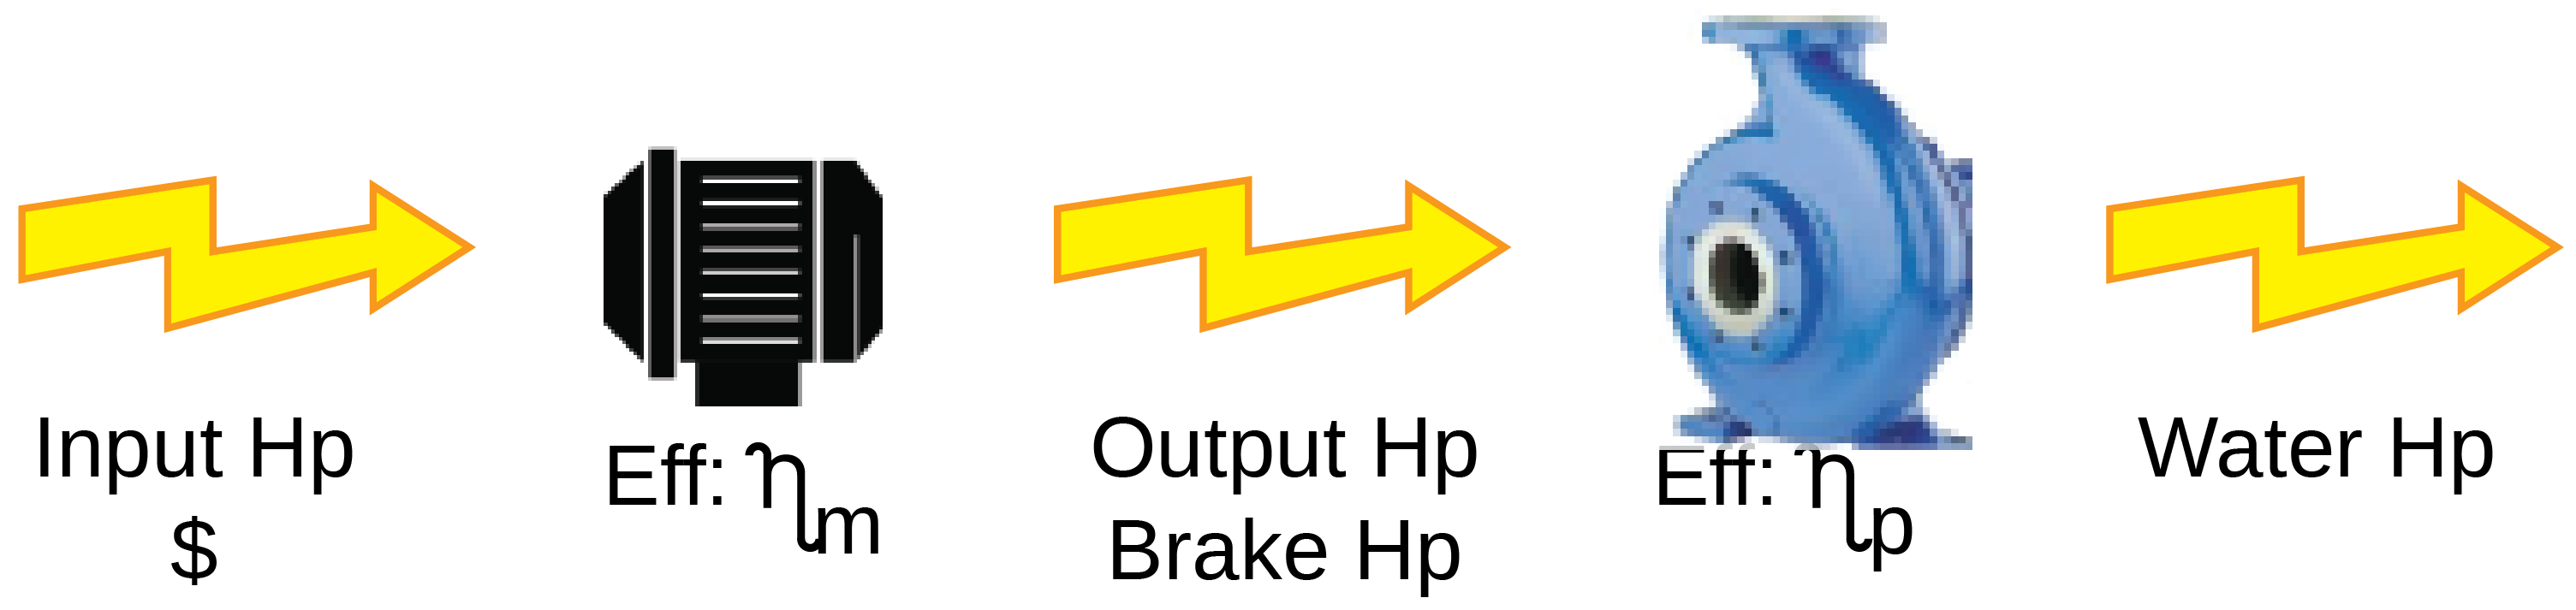
\includegraphics[scale=0.08]{PumpProblem}\\
 \vspace{0.2cm}
 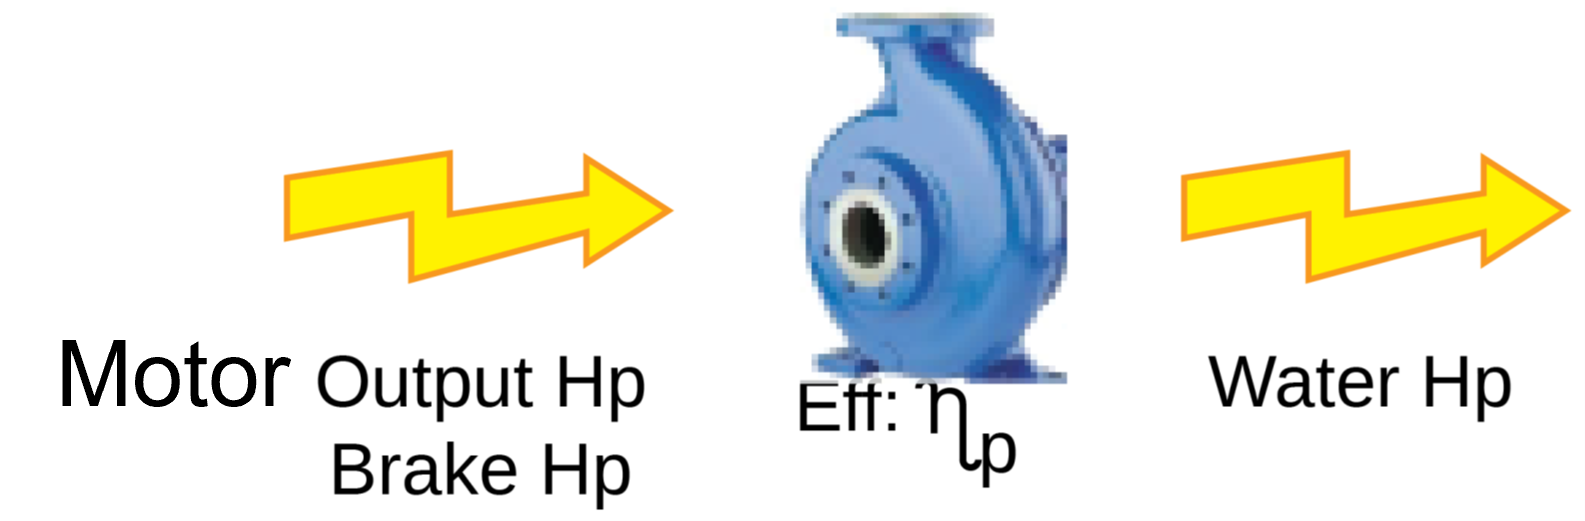
\includegraphics[scale=0.32]{PumpingProblemPump}
 $\eta_p=\dfrac{10 \mathrm{BHp}}{15.4 \mathrm{EHp}} \times 100=\boxed{65 \%}$
 \vspace{0.2cm}
 
 
 Solution:\\
  \vspace{0.2cm}
 \vspace{0.32cm}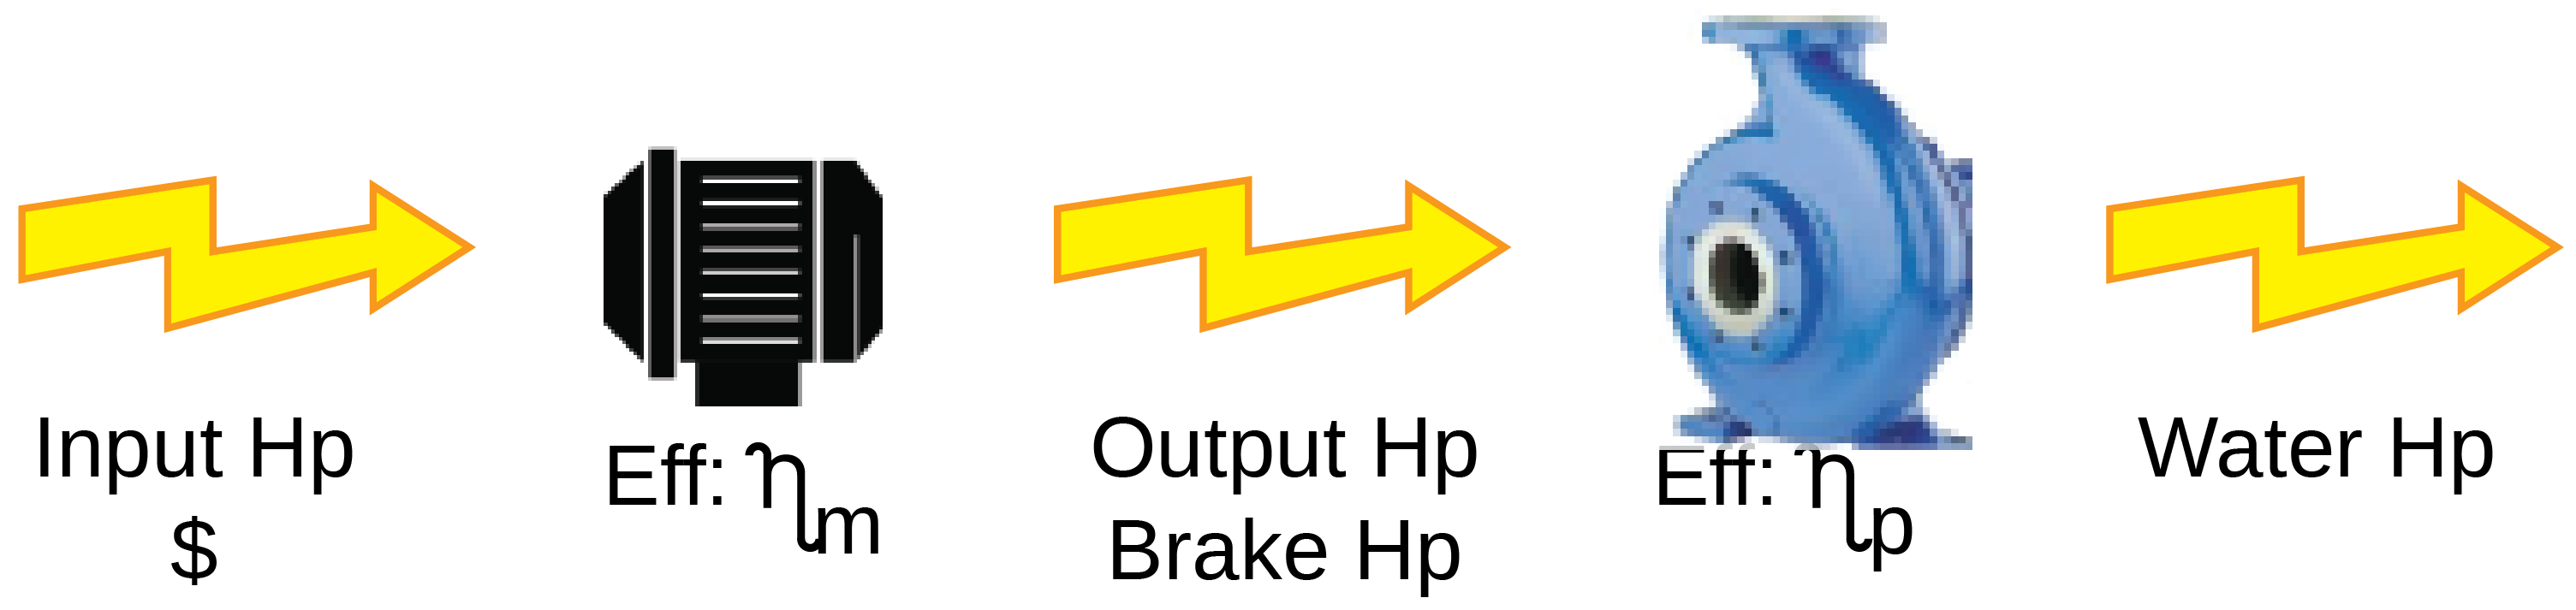
\includegraphics[scale=0.08]{PumpProblem}\\
 \vspace{0.2cm}
 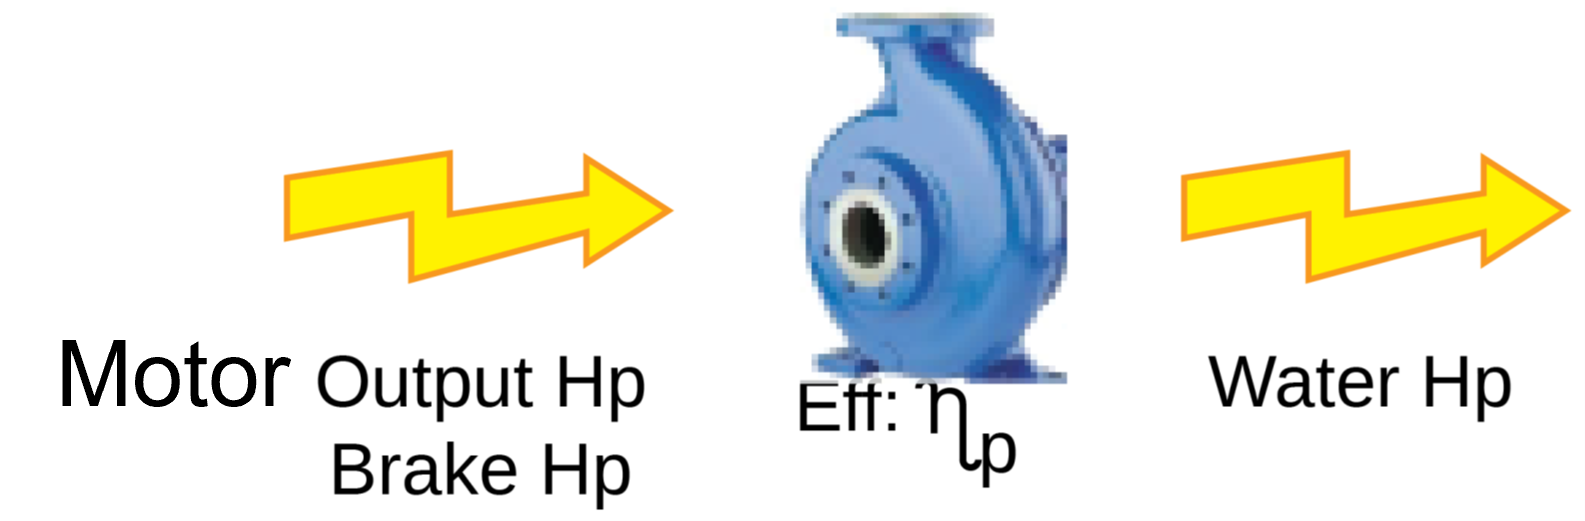
\includegraphics[scale=0.4]{PumpingProblemPump}
 \vspace{0.2cm}
$\eta_p=\dfrac{25 \mathrm{\enspace Water \enspace Hp}}{48 \mathrm{\enspace brake \enspace Hp}} \times 100=\boxed{52 \%}$
  \vspace{0.4cm}
 Solution:\\ 
 \vspace{0.2cm}
$Well \enspace efficiency=\eta_m * \eta_p \implies 0.94 \times 0.75=0.705 \times 100=\boxed{71 \%}$
 \vspace{0.2cm}


 Solution:\\
 \vspace{0.4cm}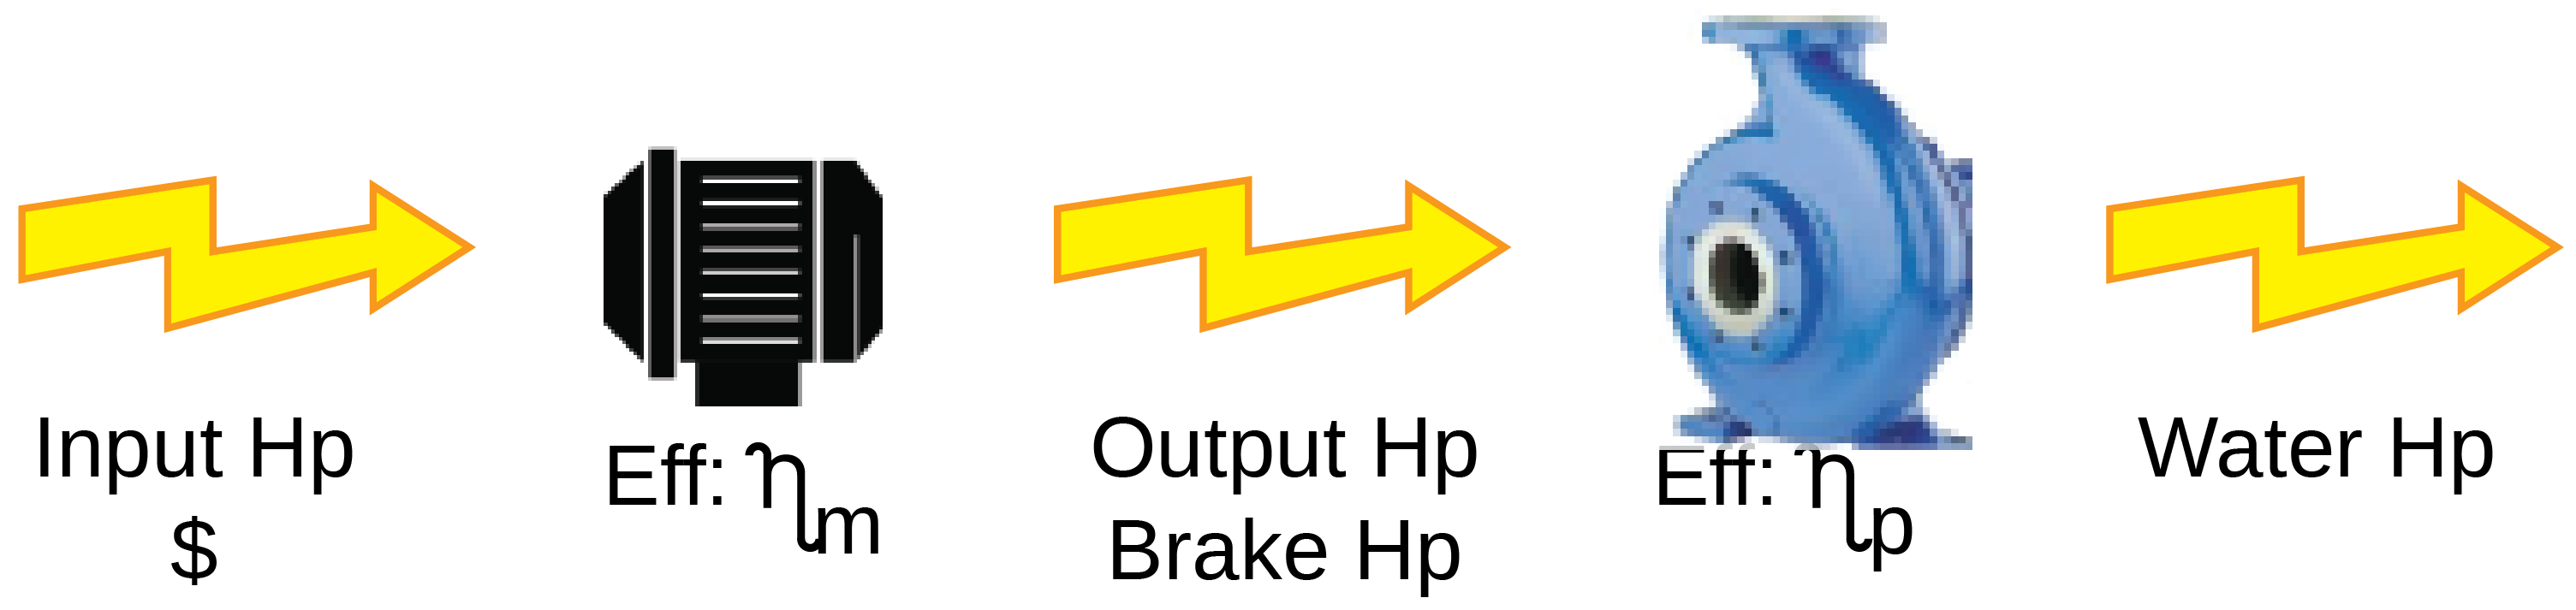
\includegraphics[scale=0.08]{PumpProblem}\\
 \vspace{0.2cm}
 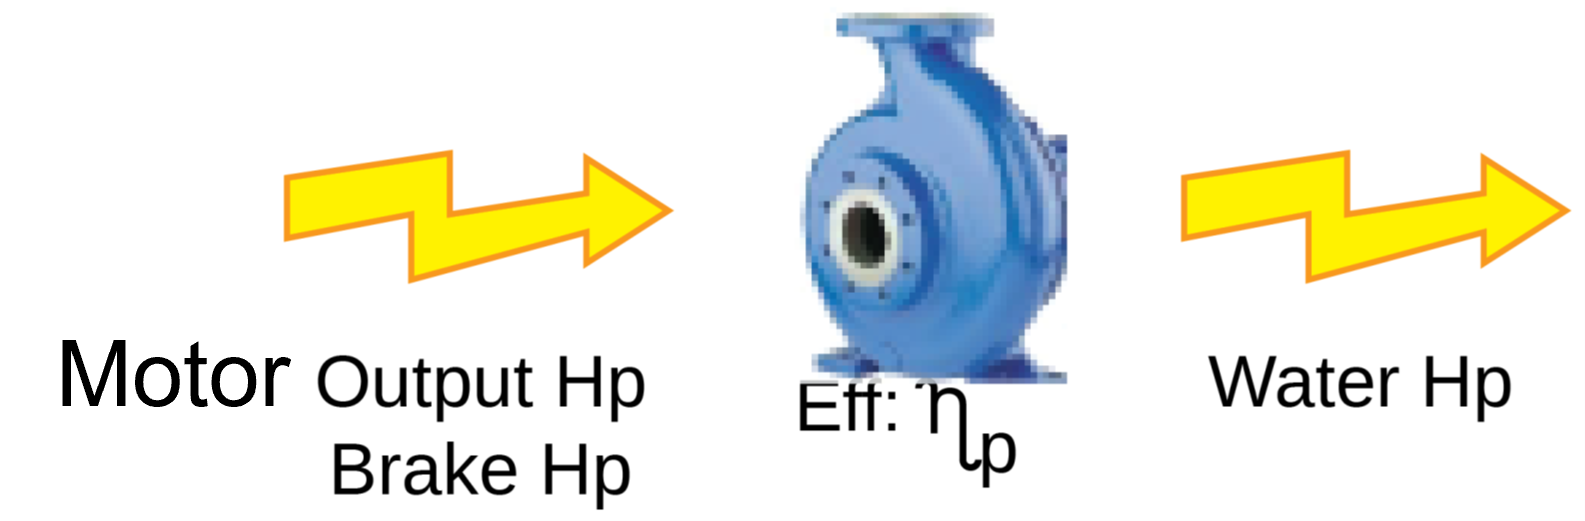
\includegraphics[scale=0.32]{PumpingProblemPump}
 \vspace{0.2cm}
$\dfrac{10 \mathrm{BHp}}{0.85}=\boxed{12 \mathrm{EHp \enspace or \enspace Input \enspace Hp}}$
 \vspace{0.4cm}


  Solution:\\ 
  \vspace{0.2cm}
 \vspace{0.08cm}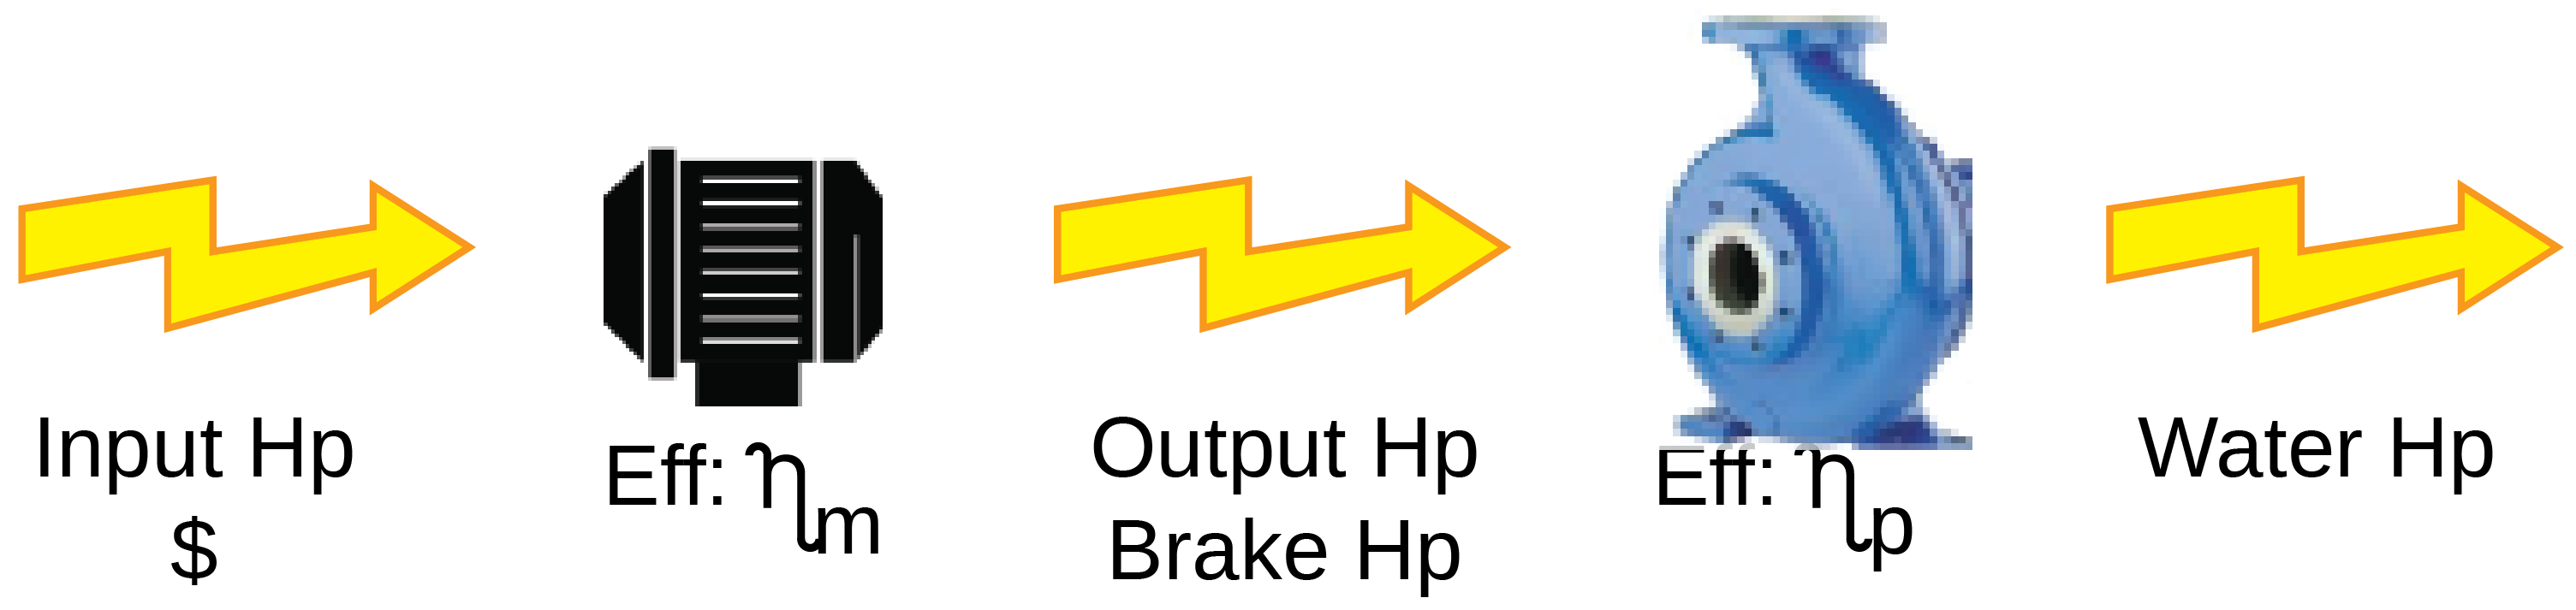
\includegraphics[scale=0.08]{PumpProblem}\\
 \vspace{0.2cm}
 \includegraphics[scale=0.32]{PumpingProblempump}
 \vspace{0.2cm}
$\eta_p=\dfrac{8.2 \mathrm{\enspace W \enspace Hp}}{10.3 \mathrm{\enspace BHp}} \times 100=\boxed{80 \%}$
 \vspace{0.2cm}


Solution:\\
\vspace{0.4cm}
water Hp = flow * head\\
\vspace{0.4cm}
$\mathrm{Water} \enspace \mathrm{Hp} = 120 \enspace \mathrm{gpm}*1,200 \enspace ft*\dfrac{\mathrm{Hp}}{3,960 \enspace \mathrm{gpm-ft}}=\boxed{ 37 \enspace \mathrm{Hp}}$\\
\vspace{0.2cm}


Solution:\\
\vspace{0.4cm}
$25 \enspace \mathrm{Hp}\dfrac{0.746 \enspace \mathrm{kW}}{\mathrm{Hp}}*\dfrac{8 \enspace \mathrm{hrs}}{\mathrm{day}}*\dfrac{7 \enspace \mathrm{days}}{\mathrm{month}}*\dfrac{\$0.07}{\mathrm{kWh}}=\boxed{\dfrac{\$73.1}{\mathrm{week}}}$\\
\vspace{0.2cm}

 Solution:\\
 \vspace{0.4cm}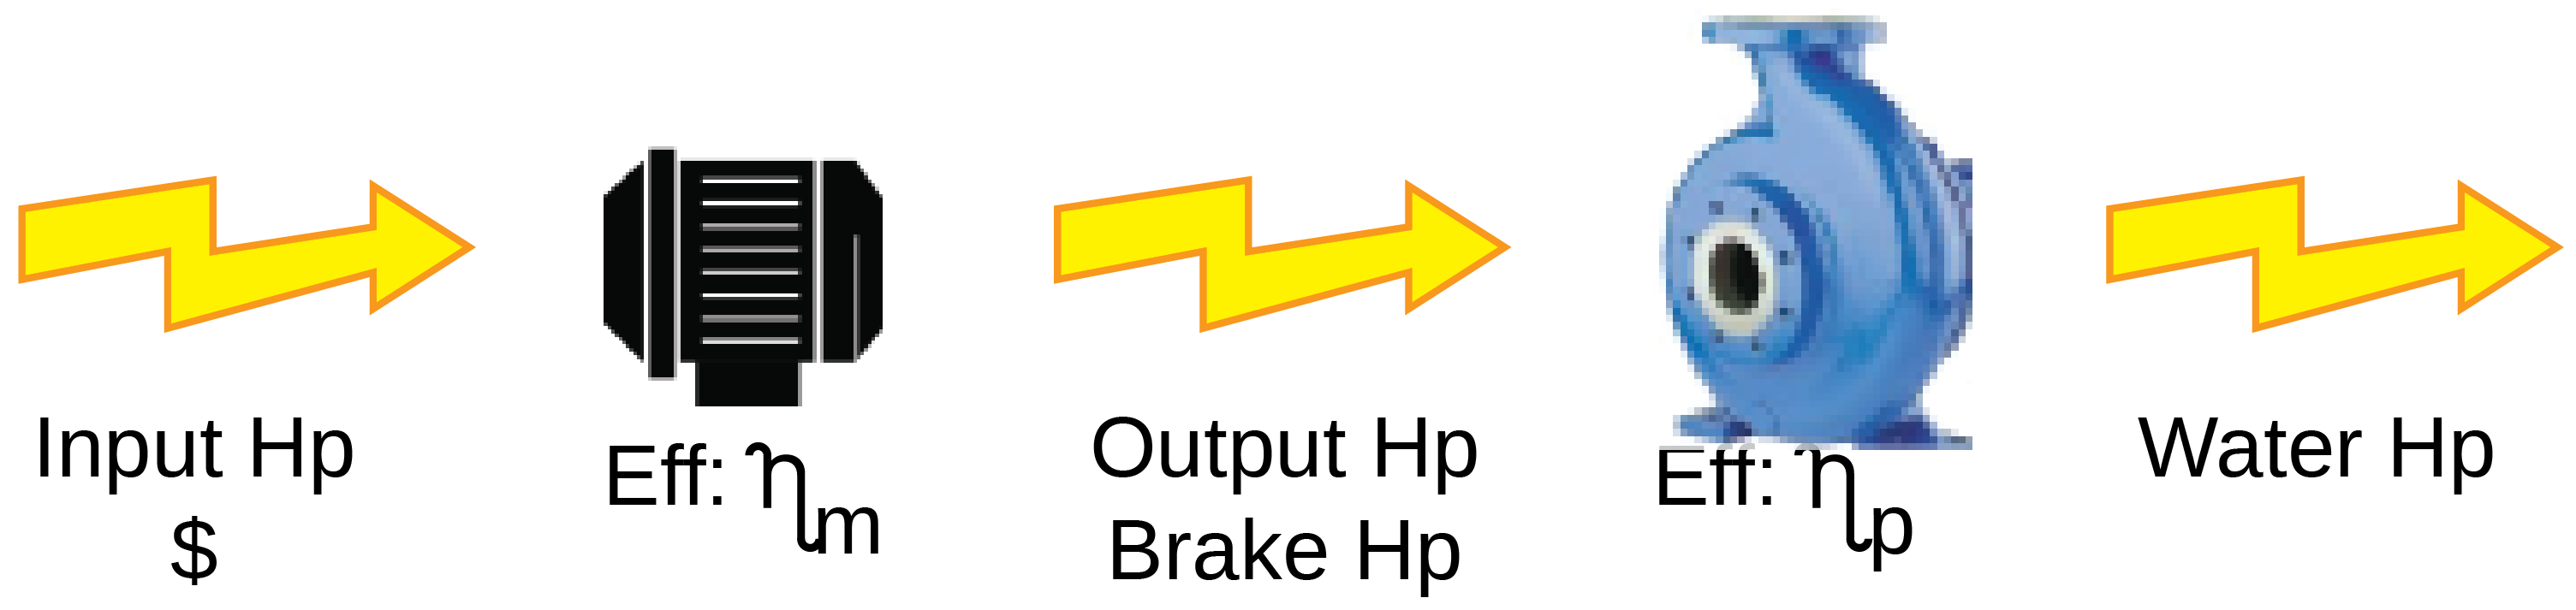
\includegraphics[scale=0.08]{PumpProblem}\\
 \vspace{0.2cm}
 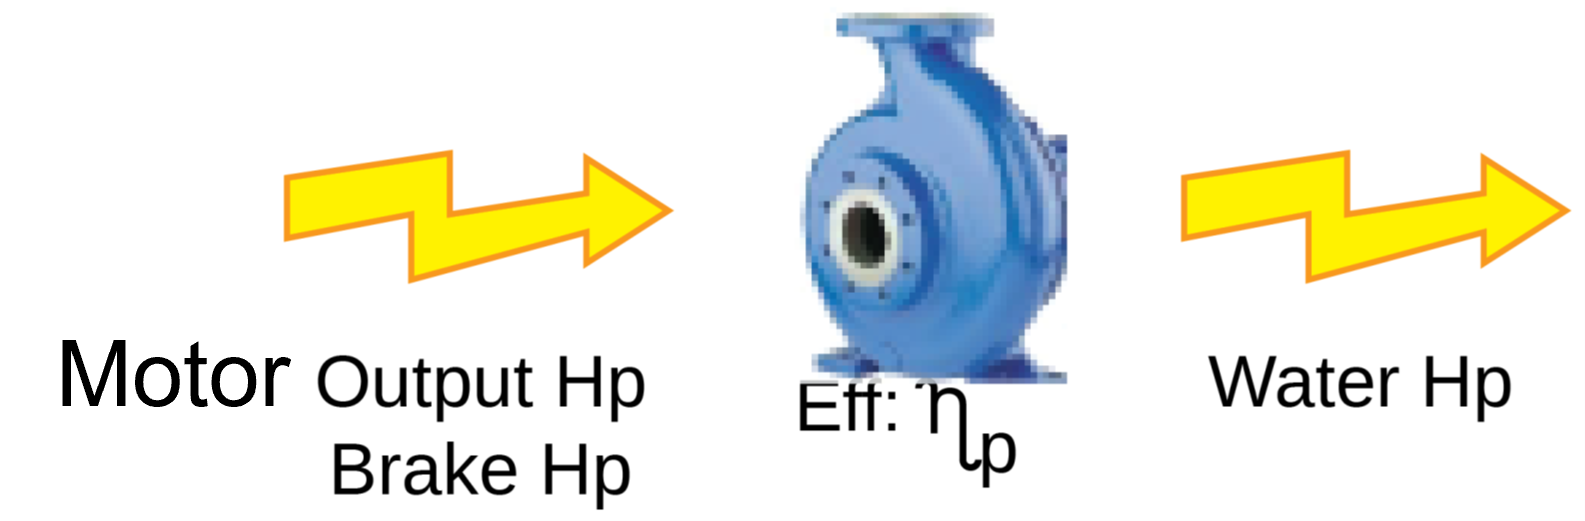
\includegraphics[scale=0.32]{PumpingProblemPump}
 \vspace{0.2cm}

water Hp = flow * head\\
 \vspace{0.2cm}
$\mathrm{Water} \enspace \mathrm{Hp} = 500 \enspace \mathrm{gpm}*50 \enspace ft*\dfrac{\mathrm{Hp}}{3,960 \enspace \mathrm{gpm-ft}}=\boxed{ 6.3 \enspace \mathrm{WHp}}$\\ 
  \vspace{0.2cm}
$\mathrm{Pump \enspace efficiency} =\dfrac{\mathrm{water \enspace Hp}}{\mathrm{brake \enspace Hp}} \implies \mathrm{brake \enspace Hp}=\dfrac{\mathrm{pump \enspace Hp}}{\mathrm{Pump \enspace efficiency}}$ \\
  \vspace{0.2cm}
$\textrm{brake} \enspace Hp = \dfrac{6.3}{0.85}=\boxed{7.4 \enspace \mathrm{Hp}}$\\
  \vspace{0.2cm}
$\mathrm{Motor \enspace efficiency} =\dfrac{\mathrm{brake \enspace Hp}}{\mathrm{input \enspace Hp}} \implies \mathrm{input \enspace \enspace Hp}=\dfrac{\mathrm{brake \enspace Hp}}{\mathrm{motor \enspace efficiency}}= \dfrac{7.4}{0.9}=\boxed{8.2 \enspace \mathrm{Hp}}$\\
  \vspace{0.2cm}
  
 \vspace{0.2cm}
$\mathrm{Wire-to-water} \enspace \mathrm{efficiency}=\eta_m * \eta_p \implies 0.9 \times 0.85 \times 100=\boxed{77 \%}$

 Solution:\\
\vspace{0.4cm}
water Hp = flow * head\\
$150 \enspace \mathrm{GPM}*75\mathrm{ft}*\dfrac{Hp}{3,960 GPM-ft}=\boxed{Water \enspace Hp = 2.8Hp}$\\
\vspace{0.4cm}
pump Hp = brake Hp * pump efficiency\\
$brake \enspace Hp = \dfrac{2.8}{0.9}=\boxed{Brake \enspace Hp=3.1Hp}$
 \vspace{0.2cm}




\section*{Practice Problems - Chemical Dosing}


  Determine the chlorinator setting in pounds per day if a water plant produces $300 \mathrm{gpm}$ and the desired chlorine dose is $2.0 \mathrm{mg} / \mathrm{L}$.

  The finished water chlorine demand is $1.2 \mathrm{mg} / \mathrm{L}$ and the target residual is $2.0 \mathrm{mg} / \mathrm{L}$. If the plant flow is $5.6 \mathrm{mgd}$, how many pounds per day of $65 \%$ hypochlorite solution will be required?

  Fluoride is added to finished water at a dose of $4 \mathrm{mg} / \mathrm{L}$. Find the feed rate setting for a fluoride saturator in gal/min if the water plant produces $5 \mathrm{mgd}$.

  If chlorine costs $\$ 0.21$ per pound, what is the daily cost to chlorinate a $5 \mathrm{mgd}$ flow rate at a dosage of $2.6 \mathrm{mg} / \mathrm{L}$ ?

  One gallon of sodium hypochlorite laundry bleach, with $5.25 \%$ available chlorine, contains how many pounds of active chlorine?

  How much sodium hypochlorite, in gallons, is required to obtain a residual of $100 \mathrm{mg} / \mathrm{L}$ in a well? The casing diameter is 18 -inches and the length is 80 feet. Sodium hypochlorite contains 5.25\% available chlorine. Assume a demand of $15 \mathrm{mg} / \mathrm{L}$.

  A water company uses an average of $600 \mathrm{gpm}$ of water. The water contains $0.30 \mathrm{mg} / \mathrm{L}$ of manganese and $0.06 \mathrm{mg} / \mathrm{L}$ of iron. How many pounds of iron and manganese are pumped into the distribution system each year?

  How many pounds of copper sulfate will be needed to dose a reservoir with $0.6 \mathrm{mg} / \mathrm{L}$ of copper? The reservoir holds 30 million gallons. The copper sulfate is $25 \%$ copper by weight.

  Liquid alum delivered to a water treatment plant contains $642.3$ milligrams of aluminum per milliliter of liquid solution. Jar tests indicate that the best alum dose is $9 \mathrm{mg} / \mathrm{L}$. Determine the setting on the liquid alum feeder in $\mathrm{ml} / \mathrm{min}$ when the plant flow is $3.2 \mathrm{mgd}$.

  The raw water supply contains $1.8 \mathrm{mg} / \mathrm{L}$ of fluoride. The flow rate is $400 \mathrm{gpm}$. The target fluoride dose for the finished water is $3 \mathrm{mg} / \mathrm{L}$. Find the desired feed rate in gpm for a fluoride saturator.

  The raw water alkalinity is $50 \mathrm{mg} / \mathrm{L}$ as calcium carbonate. The water is treated by adding 15 $\mathrm{mg} / \mathrm{L}$ of alum. What is the alkalinity of the finished water?



\section*{Practice Problems - Blending and Dilution}


Ferric chloride is being added as a coagulant to the raw water entering a plant. Sampling
shows that the concentration of ferric in the raw water is 25 ppm. A quick check of the chemical
metering pump shows that it is operating at a flow rate of 4.3 gpm. If the flow through the water
plant is 800 gpm, what is the concentration of raw chemical in the dosing tank?

A water plant is fed by two different wells. The first well produces water at a rate of 600
gpm and contains arsenic at 0.5 mg/L. The second well produces water at a rate of 350 gpm and
contains arsenic at 12.5 mg/L. What is the arsenic concentration of the blended water?

Liquid polymer is delivered as an 8 percent solution. How many gallons of liquid polymer
should be mixed in a tank to produce 150 gallons of 0.6 percent solution?

There are two raw water lines feeding a water plant. One line carries a flow rate of 500 gpm
with a TDS concentration of 1500 mg/L. The second line has a flow rate of 6 mgd with a a 250
mg/L TDS concentration. What is the actual combined TDS concentration entering the plant?


\textbf{Solutions:}\\

Solution:\\
\vspace{0.3cm}
\begin{tikzpicture}

\draw [-] (-3.2,4.2) -- (-0.4,4.2);
\draw [->] (-0.2,4) -- (-0.2,1.9);
\draw [->] (-3.2,1.9) -- (4,1.9);
\draw [shift={(-0.4,4)}] plot[domain=0:1.57,variable=\t]({1*0.2*cos(\t r)+0*0.2*sin(\t r)},{0*0.2*cos(\t r)+1*0.2*sin(\t r)});
\draw (-3.1,4.1) node[anchor=north west] {V$_{\tiny{FeCl_3}}$=$4.3 gpm$};
\draw (-3.1,3.6) node[anchor=north west] {C$_{\tiny{FeCl_3}}$ = ?};
\draw (-4.2,4.5) node[anchor=north west] {FeCl$_3$};
\draw (-4.2,2.2) node[anchor=north west] {Water};
\draw (-2.1,1.8) node[anchor=north west] {$800 gpm$};
\draw (0.7,1.8) node[anchor=north west] {C$_2$=25ppm FeCl$_3$};
\draw (0.7,1.3) node[anchor=north west] {V$_2$=4.3+800=804.3 gpm};
\end{tikzpicture}\\
\vspace{0.2cm}
C$_1$ * V$_1$ = C$_2$ * V$_2$ \\
\vspace{0.2cm}
C$_{\tiny{FeCl_3}}$ * V$_{\tiny{FeCl_3}}$  =  C$_2$ * (V$_{\tiny{FeCl_3}}$+V$_{\tiny{Water}}$)\\
\vspace{0.2cm}
C$_{\tiny{FeCl_3}}$ * 4.3 =  25 * (804.3)\\
\vspace{0.2cm}
C$_{\tiny{FeCl_3}}=\dfrac{25 * (804.3)}{4.3}=\boxed{4,676 \enspace \mathrm{ppm} \enspace \mathrm{or} \enspace 0.47\%}$\\
\vspace{0.3cm}

Solution:\\
\vspace{0.2cm}
C$_1$ * V$_1$ + C$_2$ * V$_2$ + =  C$_3$ * V$_3$=C$_3$*(V$_1$ + V$_2$)\\
\vspace{0.2cm}
C$_{Well \enspace 1}$ * V$_{Well \enspace 1}$ + C$_{Well \enspace 2}$ * V$_{Well \enspace 2}$ =  C$_{Blend}$ * V$_{Blend}$=C$_{Blend}$*(V$_{Well \enspace1}$ + V$_{Well \enspace 2}$)\\
\vspace{0.3cm}
$\implies C_{Blend}=\dfrac{C_{Well \enspace 1} * V_{Well \enspace 1} + C_{Well \enspace 2} * V_{Well \enspace 2}}{V_{Well \enspace 1} + V_{Well \enspace 2}}=\dfrac{0.5*600+12.5*350}{600+350}=\boxed{4.9 \enspace \textrm{mg/l}}$


Solution:\\
\vspace{0.5cm}
\begin{tikzpicture}[scale=1]
\draw[thick,-](-2,5) -- (0,5)node [at start, below,  black]{\small{}} node [anchor=north west, black]{} node [at start, left, black] (n){Water};;

\draw[thick,->](0,5)--(0,4.3) node [left,  black]{\small{}} node [anchor=north west, green]{} node [at start, above, red] (n){};
%\tikz\draw[line width=2mm] (0,0) -- (0,4);

\draw [<->] (2,1.9) -- (2,2.3) node [midway, midway] {};

\draw [<->] (-2,1.9) -- (-2,3.7) node [midway, midway] {};

\node [draw, cylinder, cylinder body fill=green, cylinder end fill=green!80, shape aspect=2, rotate=90, minimum height=1cm, minimum width=3cm] (c) at 
(0,3.8){};

%
\node [draw, cylinder, cylinder uses custom fill, cylinder body fill=black!10, 
cylinder end fill=black!10, shape aspect=2, rotate=90, minimum height=2cm, minimum width=3cm] (c1) at 
(0,2.8){};
%

\node [draw, cylinder, cylinder uses custom fill, cylinder body fill=black!30, 
cylinder end fill=black!10, shape aspect=2, rotate=90, minimum height=0.5cm, minimum width=3cm] (c1) at 
(0,2){};

\draw (2.2,2.6) node[anchor=north west] {C$_{1}$=8\%};

\draw (2.2,2.2) node[anchor=north west] {V$_{1}$=?};

\draw (-4,3.3) node[anchor=north west] {C$_{2}$=0.6\%};

\draw (-4,2.8) node[anchor=north west] {V$_{2}$=150 gal};



%\coordinate(dhtop) at ($(c1.after top)!-1*.1!(c1.before top)$);
%\coordinate(dhbot) at ($(c1.before bottom)!-1*.1!(c1.after bottom)$);
%\coordinate(dhlabel) at ($(dhtop)!.5!(dhbot)$);
%%\draw[|-|] (dhbot)--(dhtop);
%%\path (dhlabel) node[right, outer sep = 2pt] {$44'$};
%
%
%
%\coordinate(htop) at ($(c.before top)!-1*.1!(c.after top)$);
%\coordinate(hbot) at ($(c.after bottom)!-1*.1!(c.before bottom)$);
%\coordinate(hlabel) at ($(htop)!.5!(hbot)+(c.north)!.9!(c.center)$);
%
%\node [draw, cylinder, cylinder uses custom fill, cylinder body fill=black!20, 
%cylinder end fill=black!10, shape aspect=2, rotate=90, minimum height=1.5cm, minimum width=3cm] (c1) at 
%(0,-1.8){};
\end{tikzpicture}

\vspace{0.2cm}
C$_1$ * V$_1$ = C$_2$ * V$_2$ \\
\vspace{0.2cm}
V$_{1}$=$\dfrac{0.6*150}{8}=\boxed{11.25 \enspace \mathrm{gallons \enspace liquid \enspace polymer}} $\\
\vspace{0.3cm}


Solution:\\
\vspace{0.2cm}
C$_1$ * V$_1$ + C$_2$ * V$_2$ + =  C$_3$ * V$_3$=C$_3$*(V$_1$ + V$_2$)\\
\vspace{0.2cm}
C$_{Line \enspace 1 \enspace TDS} $ * V$_{Line \enspace 1}$ + C$_{Line \enspace 2 \enspace TDS}$ * V$_{line \enspace 2}$ =  C$_{Blend \enspace TDS}$ * V$_{Blend}$=C$_{Blend \enspace TDS}$*(V$_{Line \enspace1}$ + V$_{Line \enspace 2}$)\\
\vspace{0.3cm}
$\implies C_{Blend \enspace TDS}=\dfrac{C_{Line \enspace 1 \enspace TDS} * V_{Line \enspace 1 \enspace TDS} + C_{Line \enspace 2 \enspace TDS} * V_{Line \enspace 2}}{V_{Line \enspace 1} + V_{Line \enspace 2}}$\\
\vspace{0.3cm}
$\implies \dfrac{1500*\Big(\dfrac{500 \enspace gal}{min}*\dfrac{MG}{1,000,000 \enspace gal}*\dfrac{1440 min}{day}\Big)+6*250}{\Big(\dfrac{500 \enspace gal}{min}*\dfrac{MG}{1,000,000 \enspace gal}*\dfrac{1440 min}{day}\Big)+6}=\boxed{384 \enspace \textrm{mg/l}}$



\section*{Practice Problems - Sedimentation}


A circular clarifier has a diameter of 80 ft. If the flow to the clarifier is 1800 gpm, what is the surface overflow rate in gpm/ft

A sedimentation basin 70 ft by 25 ft receives a flow of 1000 gpm. What is the surface overflow rate in gpm/ft$2$?


A circular clarifier receives a flow of 3.55 MGD. If the diameter of the weir is 90 ft, what is the weir loading rate in gpm/ft?


\textbf{Solution}

$\mathrm{Surface \enspace overflow \enspace rate}=\dfrac{\mathrm{Flow, \enspace gpm}}{\mathrm{Clarifier \enspace surface \enspace area, \enspace ft}^2}=\dfrac{1,800 \enspace \mathrm{gpm}}{(0.785*80^2 )\mathrm{ft}^2}=\boxed{0.36 \enspace \mathrm{gpm/ft}^2}$

\vspace{0.2cm}
$\mathrm{Surface \enspace overflow \enspace rate}=\dfrac{\mathrm{Flow, \enspace gpm}}{\mathrm{Clarifier \enspace surface \enspace area, \enspace ft}^2}=\dfrac{1,000 \enspace \mathrm{gpm}}{(70 \mathrm{ft} \enspace * 25 \mathrm{ft})\mathrm{ft}^2}=\boxed{0.6 \enspace \mathrm{gpm/ft}^2}$

\vspace{0.2cm}
$\mathrm{Weir \enspace overflow \enspace rate}=\dfrac{\mathrm{Flow, \enspace gpm}}{\mathrm{Weir} \enspace \mathrm{length} \enspace ft}$\\
\vspace{0.3cm}
$\implies \dfrac{ \dfrac{3.55 \enspace \mathrm{MG}}{\mathrm{day}}*\dfrac{1,000,000 \enspace \mathrm{gal}}{\mathrm{MG}}*\dfrac{\mathrm{day}}{1440 \enspace \mathrm{min}}}{ (3.14*90) \enspace \mathrm{ft}}=\boxed{2,465 \enspace  \mathrm{gpm/ft}}$\\
\vspace{0.3cm}
\textit{Note: The concentration and volume (or flow) units need to be the same.  Thus, the gpm flow rate of Line 1 was converted to math the MGD flow rate unit of Line 2.}







\section*{Practice Problems - Filtration}

	At an average flow of 4,000 gpm, how long of a filter run in hours would be required to produce 25 MG of filtered water?
	
	A filter is $40 \mathrm{ft}$ long by $20 \mathrm{ft}$ wide. During a test of flow rate, the influent valve to the filter is closed for 6 minutes. The water level drop during this period is 16 inches. What is the filtration rate for the filter in $\mathrm{gpm} / \mathrm{ft}^{2}$ ?\\

  A water plant has three filters. Each filter is 12 feet wide by 12 feet long. Find the hydraulic loading rate in gpm/sf when all three filters are on-line and the raw water enters the plant at $9.5$ mgd.

  A sand filter will be backwashed at a rate of $8 \mathrm{gpm} / \mathrm{sf}$. If the filter is 10 feet wide by 15 feet long, what will the filter backwash rise rate be in inches per minute?

  A series of filters must be backwashed. Each filter is 20 feet square. If the goal is to achieve a filter backwash rise rate of 30 inches per minute, what should the backwash rate be in gpm/sf?

  A water plant has 3 filters. The plant is currently treating $5 \mathrm{mgd}$. If each filter is 12 feet wide by 20 feet long, what is the minimum number of filters that should be placed into service to keep the hydraulic loading rate below 20 gpm/sf?

  Find the yield for a filter in lbs/hr/sf given the following information: Filter operates for 12 hours of each day and captures $95 \%$ of the influent solids. The solids load to the filter is 200 pounds per day. The filter is 40 feet square.

  Coagulated raw water contains $120 \mathrm{mg} / \mathrm{L}$ of total suspended solids. The water plant produces $2.0 \mathrm{mgd}$ and has two sand filters that are 20 feet wide by 20 feet long. If the filters operate 22 hours of each day and capture $99 \%$ of the coagulated solids, what is the filter yield in lbs/hr/sf? What is the filter yield total in pounds per day?

  A series of filters discharge into a combined effluent trough. The trough is 5 feet wide by 80 feet long. A weir runs the full length of the trough. If the water plant capacity is 2 mgd, what is the weir overflow rate in gpd/sf?



\textbf{Solution}


$Flow \enspace rate \enspace (gpm)=\dfrac{Total \enspace flow \enspace (gal)}{Filter \enspace run \enspace time \enspace (min)}$

\vspace{0.3cm}

$\implies Filter \enspace run \enspace time \enspace (min)=\dfrac{Total \enspace flow \enspace (gal)}{Flow \enspace rate \enspace (gpm)}$\\

\vspace{0.3cm}

$\implies Filter \enspace run \enspace time \enspace (hr)=25 \enspace MG*\dfrac{1,000,000 \enspace \cancel{gal}}{MG}*\dfrac{\cancel{min}}{4,000 \enspace \cancel{gal}}*60 \enspace \dfrac{hr}{\cancel{min}}=\boxed{104 \enspace hrs}$

The volume of the water dropped after the inlet valve was closed would be the filter flow rate.  Since the dimensions to calculate are in feet and inches, the volume needs to be converted from ft$^3$ to gallons\\
\vspace{0.2cm}
$\text{Filtration rate, } \mathrm{gpm} / \mathrm{ft}^{2} = 
\dfrac{(
40 \mathrm{ ft}*20 \mathrm{ ft} * 16 \mathrm{\cancel{in}}*
\dfrac{ft}{12 \enspace \cancel{in}}
)
\cancel{ft^3}*7.48 \enspace 
\dfrac
{gal}
{\cancel{ft^3}}}
{40 \enspace ft * 20 \enspace feet}= \boxed{1.7\enspace gpm/ft^2}$\\

